\documentclass[a4paper, 12pt]{article}

\usepackage[utf8]{inputenc}
\usepackage[ngerman]{babel}
\usepackage[a4paper, margin=2cm]{geometry}
\usepackage{graphicx}
\usepackage{hyperref}
\usepackage{glossaries}
\usepackage{dirtytalk}
\usepackage{tabularx}
\usepackage{hyperref}
\usepackage[table]{xcolor}
\usepackage{svg}
\usepackage{amsmath}
\usepackage{listings}
\usepackage{enumitem}
\usepackage{float}


\lstdefinelanguage{JavaScript}{
  keywords={typeof, new, true, false, catch, function, return, null, catch, switch, var, if, in, while, do, else, case, break},
  keywordstyle=\color{blue}\bfseries,
  ndkeywords={class, export, boolean, throw, implements, import, this},
  ndkeywordstyle=\color{darkgray}\bfseries,
  identifierstyle=\color{black},
  sensitive=false,
  comment=[l]{//},
  morecomment=[s]{/*}{*/},
  commentstyle=\color{purple}\ttfamily,
  stringstyle=\color{red}\ttfamily,
  morestring=[b]',
  morestring=[b]"
}

\renewcommand{\glossarysection}[2][]{}
\makeglossaries

% Section author command
\makeatletter
\newcommand{\sectionautor}[1]{
    {
        \linespread{1.1}
        \large
        \scshape
        Autor: #1
        \vspace{12pt}
    }
    \@afterheading
}
\makeatother

% Author declarations
\newcommand{\authorlukasb}{Lukas Benner}
\newcommand{\authorjonas}{Jonas Elsper}
\newcommand{\authorlukase}{Lukas Epple}

% Referenzen zu Items
\newcounter{itemcounter}[section]
\newcommand{\itm}[1]{\item[/#1/\refstepcounter{itemcounter}\label{itm-#1}]}
\newcommand{\refitm}[1]{\hyperref[itm-#1]{/#1/}}


\begin{document}
\begin{sloppypar}

\begin{titlepage}
    \begin{center}
        \vspace{0.5cm}
        
        
\includegraphics[height=2cm]{resources/htwg-logo.png}
        
        \vspace{1.5cm}

        \Huge{\textbf{Endabgabe\\}}
        \vspace{0.5cm}
        \Huge{\textbf{PARK \\ Version 1.0 \\}}
        \vspace{0.5cm}
        \Huge{\textbf{CLOUD APPLICATION DEVELOPMENT WS WS2024/25}}
    
        \vspace{1.5cm}
 
        \Large{
            \textbf{Team Merzedes} \\
            \authorjonas \\
            \authorlukasb \\
            \authorlukase
        }
 
        \vspace{1.5cm}
        
        \includegraphics[height=3.5cm]{resources/favicon.ico}

        \vspace{1.5cm}

        \large{28.10.2022}
      
    \end{center}
 \end{titlepage}

\newpage


\tableofcontents
\setcounter{page}{2}
\newpage

\section{Requirements}

PARK ist eine Software-as-a-Service (SaaS) Anwendung für die Verwaltung von Parkeinrichtungen für Gemeinden, oder Unternehmen.
Die Anwendung stellt eine umfassende Palette an Funktionen bereit, um den Parkbetrieb zu optimieren, 
die User Experience zu verbessern und die Verwaltung der Parkinfrastruktur effizienter zu gestalten.  \\


\textbf{Hauptziele:}

\begin{itemize}
    \item \textbf{Integration in die Parkinfrastruktur:} Die Anwendung wird in die Parkbereichs- und Garageninfrastruktur integriert, um die automatisierte Ein- und Ausfahrt von Fahrzeugen, sowie die Verifizierung von Zahlungen für Park- und Ladevorgänge zu ermöglichen.
    \item \textbf{Verwaltung der Parkinfrastruktur:} Die Parkinfrastrutktur wird digital abgebildet und kann flexibel an Veränderungen in der realen Welt angepasst werden. Die Integration mit den Prozessen für Parken und Laden sowie mit der Mängelverwaltung ermöglicht umfangreiche Analysen und einen ganzheitlichen Überblick über die Infrastruktur
    \item \textbf{Globale Bereitstellung:} Die SaaS Anwendung ist für globale Skalierbarkeit ausgelegt und ermöglicht eine automatisierte Bereitstellung für Kunden mit unterschiedlichen Bedürfnissen.
\end{itemize}


Funktional ermöglicht die Anwendung die digitale Abbildung der realen Infrastruktur, um die Belegung, Parkflächen, Ladestationen, Mängel und Benutzer an zentraler Stelle zu verwalten. Umfassende Benutzerverwaltung erlaubt verschiedene Sichten auf die Applikation, sodass alle Stakeholder ihren Bedürfnissen entsprechend Zugang zu unterschiedlichen Funktionen erhalten. Automatisierte Bereitstellung ermöglicht es für Tenants mit unterschiedlichen Bedürfnissen, eine auf sie zugeschnittene Instanz der Anwendung erstellen zu können.


\subsection{System Context}

Das System läuft im Kontext unterschiedlicher interner und externer Komponenten. Interne Komponenten beschreiben dabei Komponenten, die vom Solution Administrator selbst verwaltet werden, über die er/sie also eine gewisse Kontrolle hat. Externe Komponenten sind dann alle diejenigen, über die der Solution Administrator keine Kontrolle hat. 

In Abbildung \ref{fig:context-diagram} ist der Systemkontext und die Interaktion mit der Solution in einem Kontextdiagram dargestellt.

\begin{figure}[H]
    \centering
    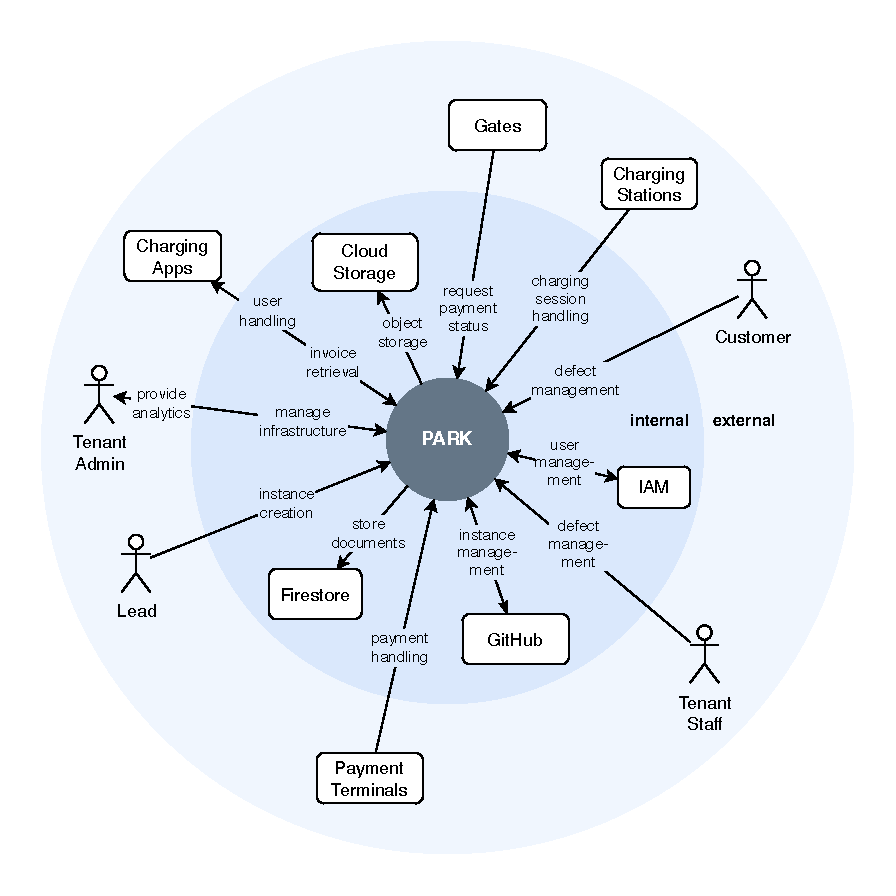
\includegraphics[width=0.9\textwidth]{resources/context-diagram.pdf}
    \caption{Context Diagram}
    \label{fig:context-diagram}
\end{figure}


\subsection{Use Case Overview}
Im folgenden Abschnitt werden die Use Cases der Parking Management Lösung genauer beschrieben. Diese Aktoren existieren in diesem Kontext:

\renewcommand{\arraystretch}{1.5}
{\rowcolors{2}{}{gray!20}
\begin{longtable}{l p{10cm}}
    \caption{Use Case Aktoren}
    \label{tab:use-case-actors} \\
    \textbf{Actor} & \textbf{Beschreibung} \\ [1ex]
    Customer & Der Endkunde, der die Parking Infrastruktur nutzt \\ [0.5ex]
    Tenant Staff & Mitarbeiter (bspw. Financial oder Operations) des Tenants \\ [0.5ex]
    Tenant Administrator & Administrator auf Tenant-Ebene \\ [0.5ex]
    Solution Administrator & Administrator, der die Lösung bereitstellt \\ [0.5ex]
    Lead & Potenzielle Kunden, die eine Instanz der Lösung erstellen möchten \\ 
\end{longtable}}

Zusätzlich zu den Aktoren, die entsprechende Personen darstellen, existieren noch sogenannte System Actors. Damit sind die Systemkomponenten gemeint, sie auch als Aktoren mit anderen Systemkomponenten interagieren. Dies sind beispielsweise externe Komponenten wie die Ladestationen, Schranken, 3rd Party Applikationen des E-Charging Anbieters, aber auch die Microservices der Lösung, die untereinander interagieren.

Das Parking Management bündelt sämtliche Funktionalität für die Abwicklung der Prozesse rund um das Parken und Laden. In Abbildung \ref{fig:park-ma-use-cases} sind die Use Cases des Parking Managements abgebildet.

\begin{figure}[H]
    \centering
    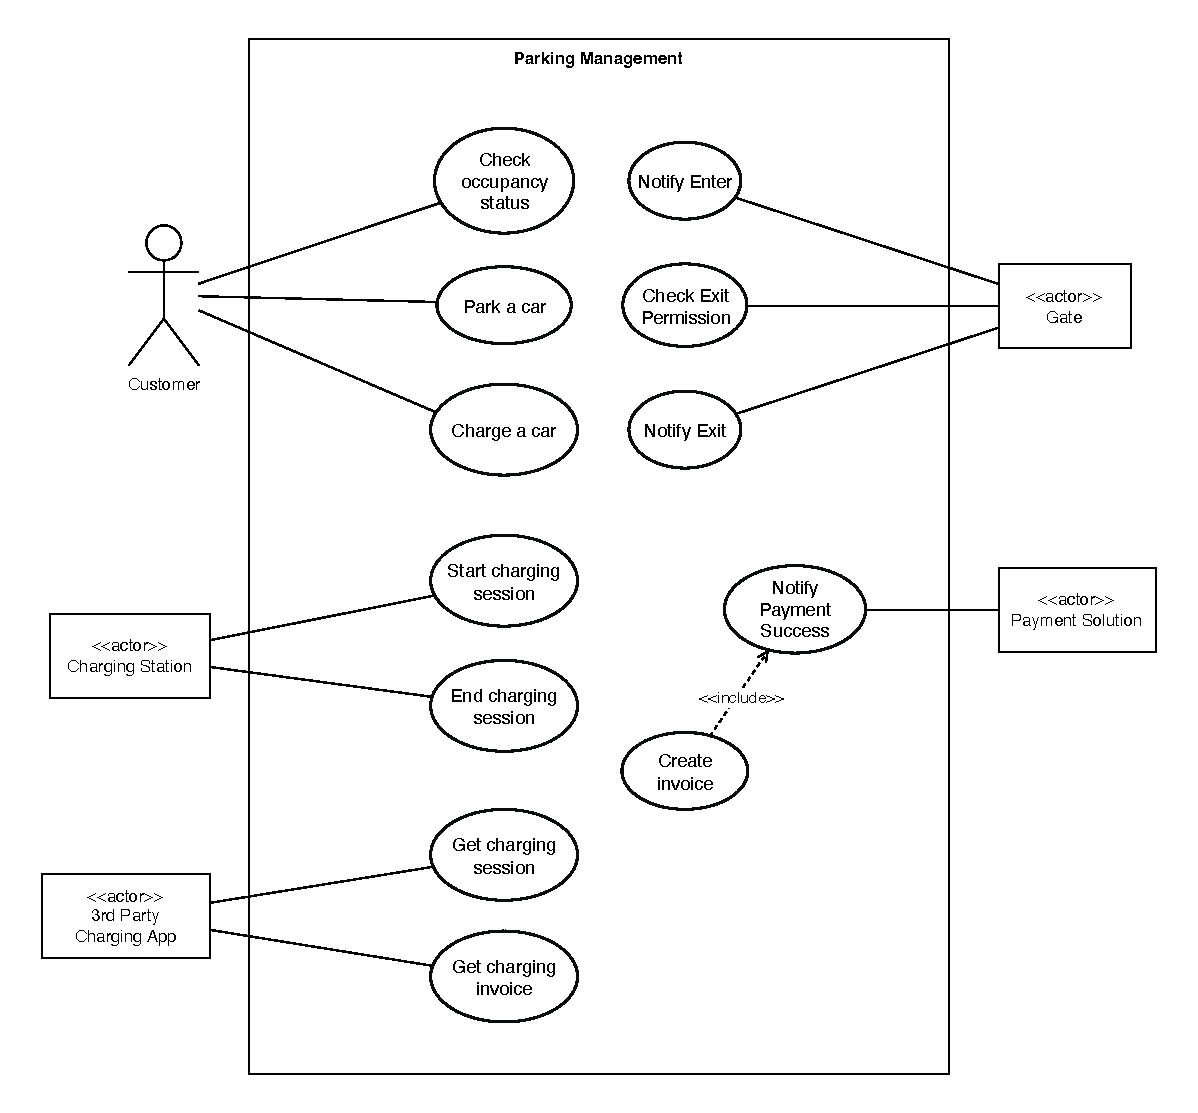
\includegraphics[width=\textwidth]{resources/park-ma-use-cases.pdf}
    \caption{Parking Management Use Cases}
    \label{fig:park-ma-use-cases}
\end{figure}

Das Property Management umfasst alle Funktionen für das Erstellen, Verwalten und Löschen der digitalen Abbildungen der Infrastruktur, sowie das Defect Management.
In Abbildung \ref{fig:prop-ma-use-cases} sind alle Use Cases für des Property Managements dargestellt.

\begin{figure}[H]
    \centering
    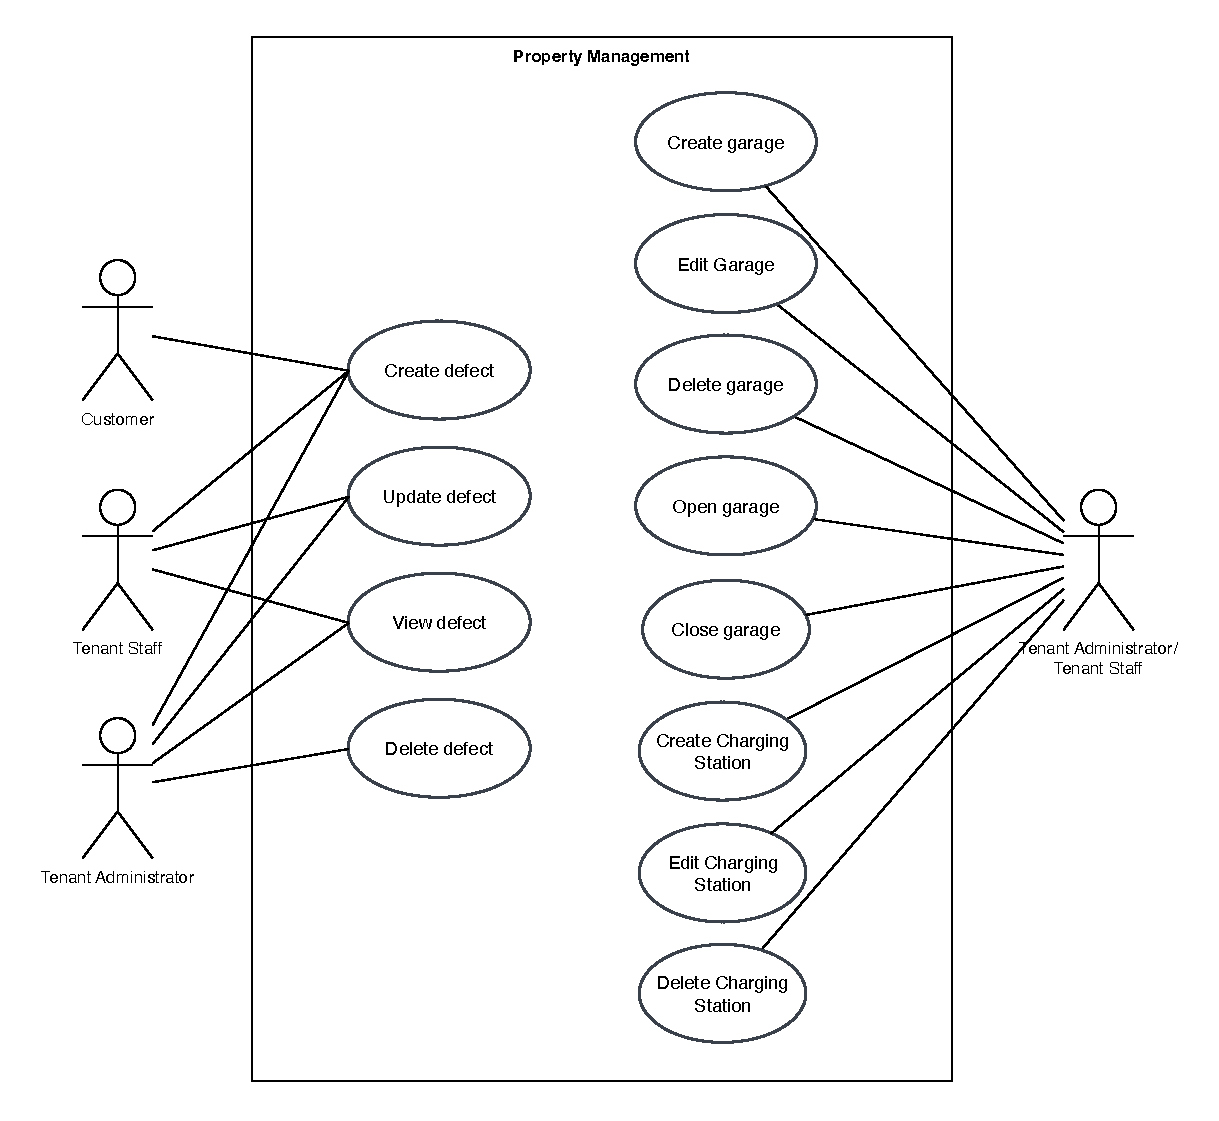
\includegraphics[width=\textwidth]{resources/prop-ma-use-cases.pdf}
    \caption{Property Management Use Cases}
    \label{fig:prop-ma-use-cases}
\end{figure}

Infrastructure Management umfasst die Verwaltung der Infrastruktur auf Anwendungsebene. Dazu gehören beispielweise die Instanzerstellung für neue Tenants und die gesamte Funktionalität für das konsolidieren und abrufen von anwendungsweiten Analytics. Abbildung \ref{fig:inf-ma-use-cases} zeigt die Use Cases für das Infrastructure Management.

\begin{figure}[H]
    \centering
    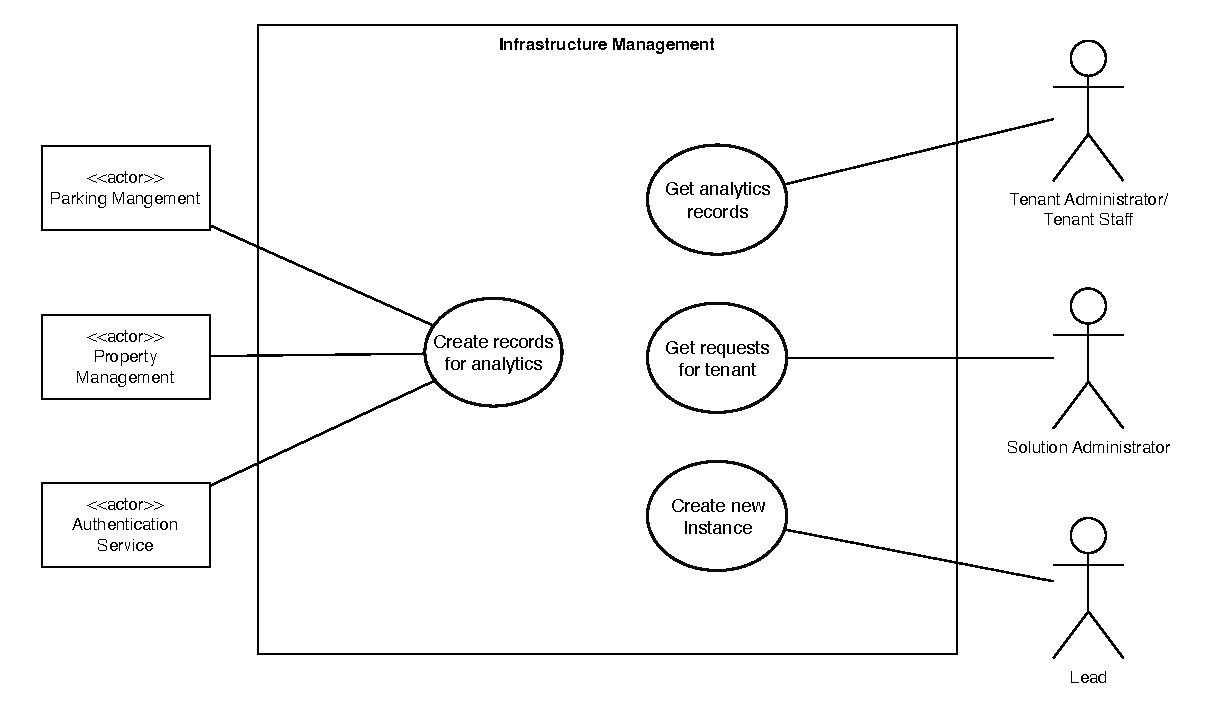
\includegraphics[width=\textwidth]{resources/inf-ma-use-cases.pdf}
    \caption{Infrastructure Management Use Cases}
    \label{fig:inf-ma-use-cases}
\end{figure}

Die Authentication Komponente der Parking Management Solution stellt einige erweiternde Funktionen zur Google Identity Platform bereit. In Abbildung \ref{fig:auth-use-cases} sind die entsprechenden Use Cases dargestellt.


\begin{figure}[H]
    \centering
    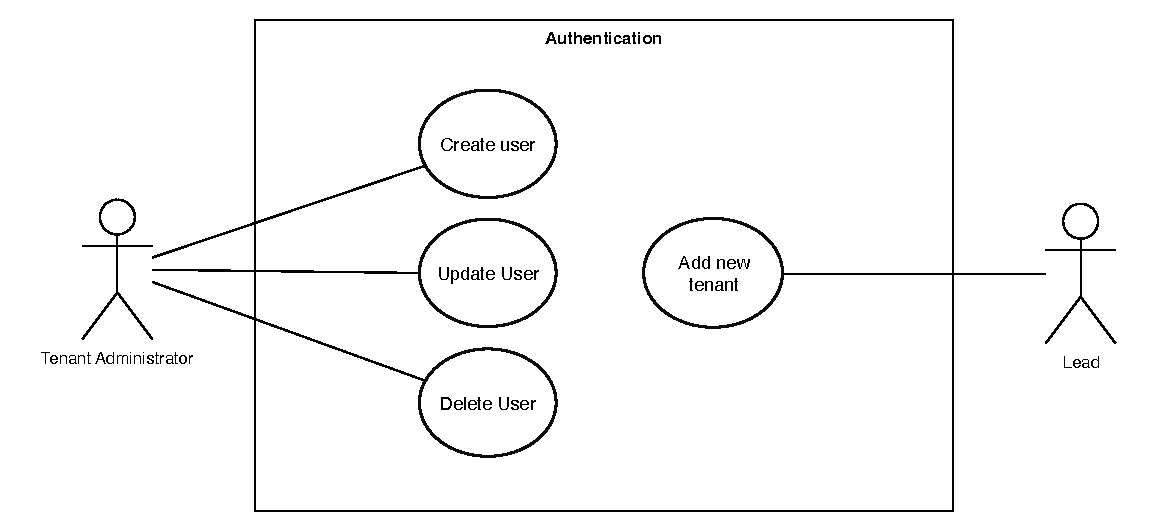
\includegraphics[width=\textwidth]{resources/auth-use-cases.pdf}
    \caption{Authentication Service Use Cases}
    \label{fig:auth-use-cases}
\end{figure}

\goodbreak
\section{Development View}

In den folgenden Abschnitten wird die Sicht auf die Anwendung während der Entwicklung beschrieben. Dies umfasst die Organisation des Quellcodes, die entwickelten Komponenten, Verwendete APIs und die Organisation der benötigten Daten.

\subsection{Software Components}

\subsubsection{Source Code Organization}
Für die Organisation unseres Quellcodes haben wir einen Monorepo-Ansatz verwendet. Alle Backend-Services, das Frontend und die Dateien für CI/CD sind in diesem Repository in der Ordnerstruktur wie in Figure \ref{fig:repo-structure} gezeigt abgelegt.

\begin{figure}[ht]
    \begin{verbatim}
        park
        |-- backend
        |   |-- authentication
        |   |   |-- ...
        |   |-- infrastructure-administration
        |   |   |-- ...
        |   |-- parking-management
        |   |   |-- ...
        |   |-- property-management
        |   |   |-- ...
        |   |-- shared
        |-- certs
        |-- ci-cd
        |   |-- helm
        |   |   |-- ...
        |   |-- terraform
        |       |-- ...
        |-- cloud-functions
        |-- docs
        |   |-- ...
        |-- frontend
        |   |-- ...
        |-- shared
        |-- signup-frontend
        |-- ...
    \end{verbatim}
    \caption{Repository Organisation}
    \label{fig:repo-structure}
\end{figure}

Für alle einzelnen Backend Microservices existiert unter \verb|backend| ein Unterordner, in dem das Node.js Projekt des entsprechenden Microservices abgelegt ist. Zusätzlich sind unter \verb|shared| TypeScript files abgelegt, die von mehreren Backend Services verwendet werden.

Der Ordner \verb|certs| ist für das lokale Testing, um dort die Key-Files der Service Accounts abzulegen.

In \verb|ci-cd| sind alle Dateien für DevOps und das Deployen der Infrastruktur abgelegt. Unter \verb|helm| liegen dabei alle Dateien, die für das Erstellen der Helm Charts benötigt werden, \verb|terraform| beinhaltet alle Konfigurationsdateien für die Cloud-Infrastruktur. Außerdem befinden noch Python-Skripte für das Deployment-Handling in diesem Verzeichnis.

Damit auch der Code für die Cloud-Functions in die Quellcodeverwaltung aufgenommen sind, existiert für diese das \verb|cloud-functions| Verzeichnis.
Unter \verb|docs| liegen einige Files für die Dokumentation ab. Darunter Skizzen für die API-Spezifikation.

Im \verb|frontend| Verzeichnis befindet sich der gesamte Client-Code der Anwendung, in diese Fall ein React Projekt mit allen Komponenten und Services des Frontends.
Außerdem existiert noch ein weiteres \verb|shared| Verzeichnis auf top-level Ebene für die DTOs zwischen Frontend und Backend.

Für die Tenant-Creation, beziehungsweise der Registrierung und Instanzerstellung für neue Tenants existiert noch ein separater Client, welcher unter \verb|signup-frontend| abgelegt ist. Hierbei handelt es sich ebenfalls um ein React-Projekt.

Während der Entwicklung haben wir mit Feature-Branches angelegt an den Git Flow gearbeitet, um eine möglichst konfliktfreie, parallele Entwicklung der Anwendung zu ermöglichen.

\subsubsection{Components}
Die Applikation umfasst 4 Microservices für das Backend:


\begin{itemize}
    \item \textbf{Authentication Service:} Erweiterung der Authentication-Funktionalität für den Kontext der Anwendung
    \item \textbf{Infrastructure Management Service:} Zentrale Verwaltung der Tenant Creation und Endpunkt zur Konsolidierung von Anwendungsweiten Analytics
    \item \textbf{Parking Management Service:} Bereitstellung der gesamten Funktionalität für das Parken, Laden und die Belegungsverwaltung
    \item \textbf{Property Management Service:} Bereitstellung der Gesamten Funktionalität für die Verwaltung der Parkinfrastruktur
\end{itemize}

Alle Backend Services sind in Node.js geschrieben, für die Bereitstellung der Web APIs wird expressjs verwendet.
Zusätzlich werden 2 Frontend Clients bereitgestellt:

\begin{itemize}
    \item \textbf{PARK Client:} Frontend für die Bedienung der Anwendung
    \item \textbf{SignUp Client:} Frontend für die Tenant-Creation/Instanzerstellung
\end{itemize}

Die Frontend Clients wurden mit React implementiert. Wie bereits im Kontextdiagram (Figure \ref{fig:context-diagram}) gezeigt, sind zudem verschiedene externe Komponenten angebunden. So werden beispielsweise unterschiedliche Komponenten aus der Google Cloud Infrastruktur verwendet (Object Storage, Firestore, Identity Platform,...). Außerdem werden extern verwaltete Komponenten angebunden, beispielsweise in Form von Schranken, Ladestationen usw. Für das automatisierte Deployment werden GitHub Actions verwendet.

\subsubsection{Libraries}
Für die Interaktion mit der Google Cloud Infrastruktur wurden unterschiedliche Libraries verwendet. Für den Zugriff auf die Firestore Infrastruktur haben wir das NPM Paket \href{hhttps://www.npmjs.com/package/firebase-admin}{firebase-admin} verwendet, welches verschiedene Methoden, beispielsweise zum Abrufen und Erstellen von Dokumenten in einer Firestore Datenbank zur Verfügung stellt.

Um Zugriff auf den Object Storage zu haben, um beispielsweise bei der Defect-Erstellung Bilder ablegen zu können haben wir den \href{https://www.npmjs.com/package/@google-cloud/storage}{google-cloud/storage} NPM Client verwendet.

Die Kommunikation mit der Google Cloud Identity Platform für das frontendseitige Anmelden ist über das \href{https://www.npmjs.com/package/@firebase/app-compat}{@firebase/app-compat package} realisiert.

Da für die Authentifizierung der Komponenten innerhalb der Anwendung JWT Tokens verwendet werden, sind außerdem die \href{https://www.npmjs.com/package/jsonwebtoken}{jsonwebtoken} Library und der OAuth2Client Client aus der \href{https://www.npmjs.com/package/google-auth-library}{google-auth-library} eingebunden.

\subsubsection{APIs}
Im Wesentlichen stellt jeder Service eine API bereit, wie in Abbildung \ref{fig:api-overview} dargestellt, über welche dessen Funktionalität genutzt werden kann.

\begin{figure}[ht]
    \centering
    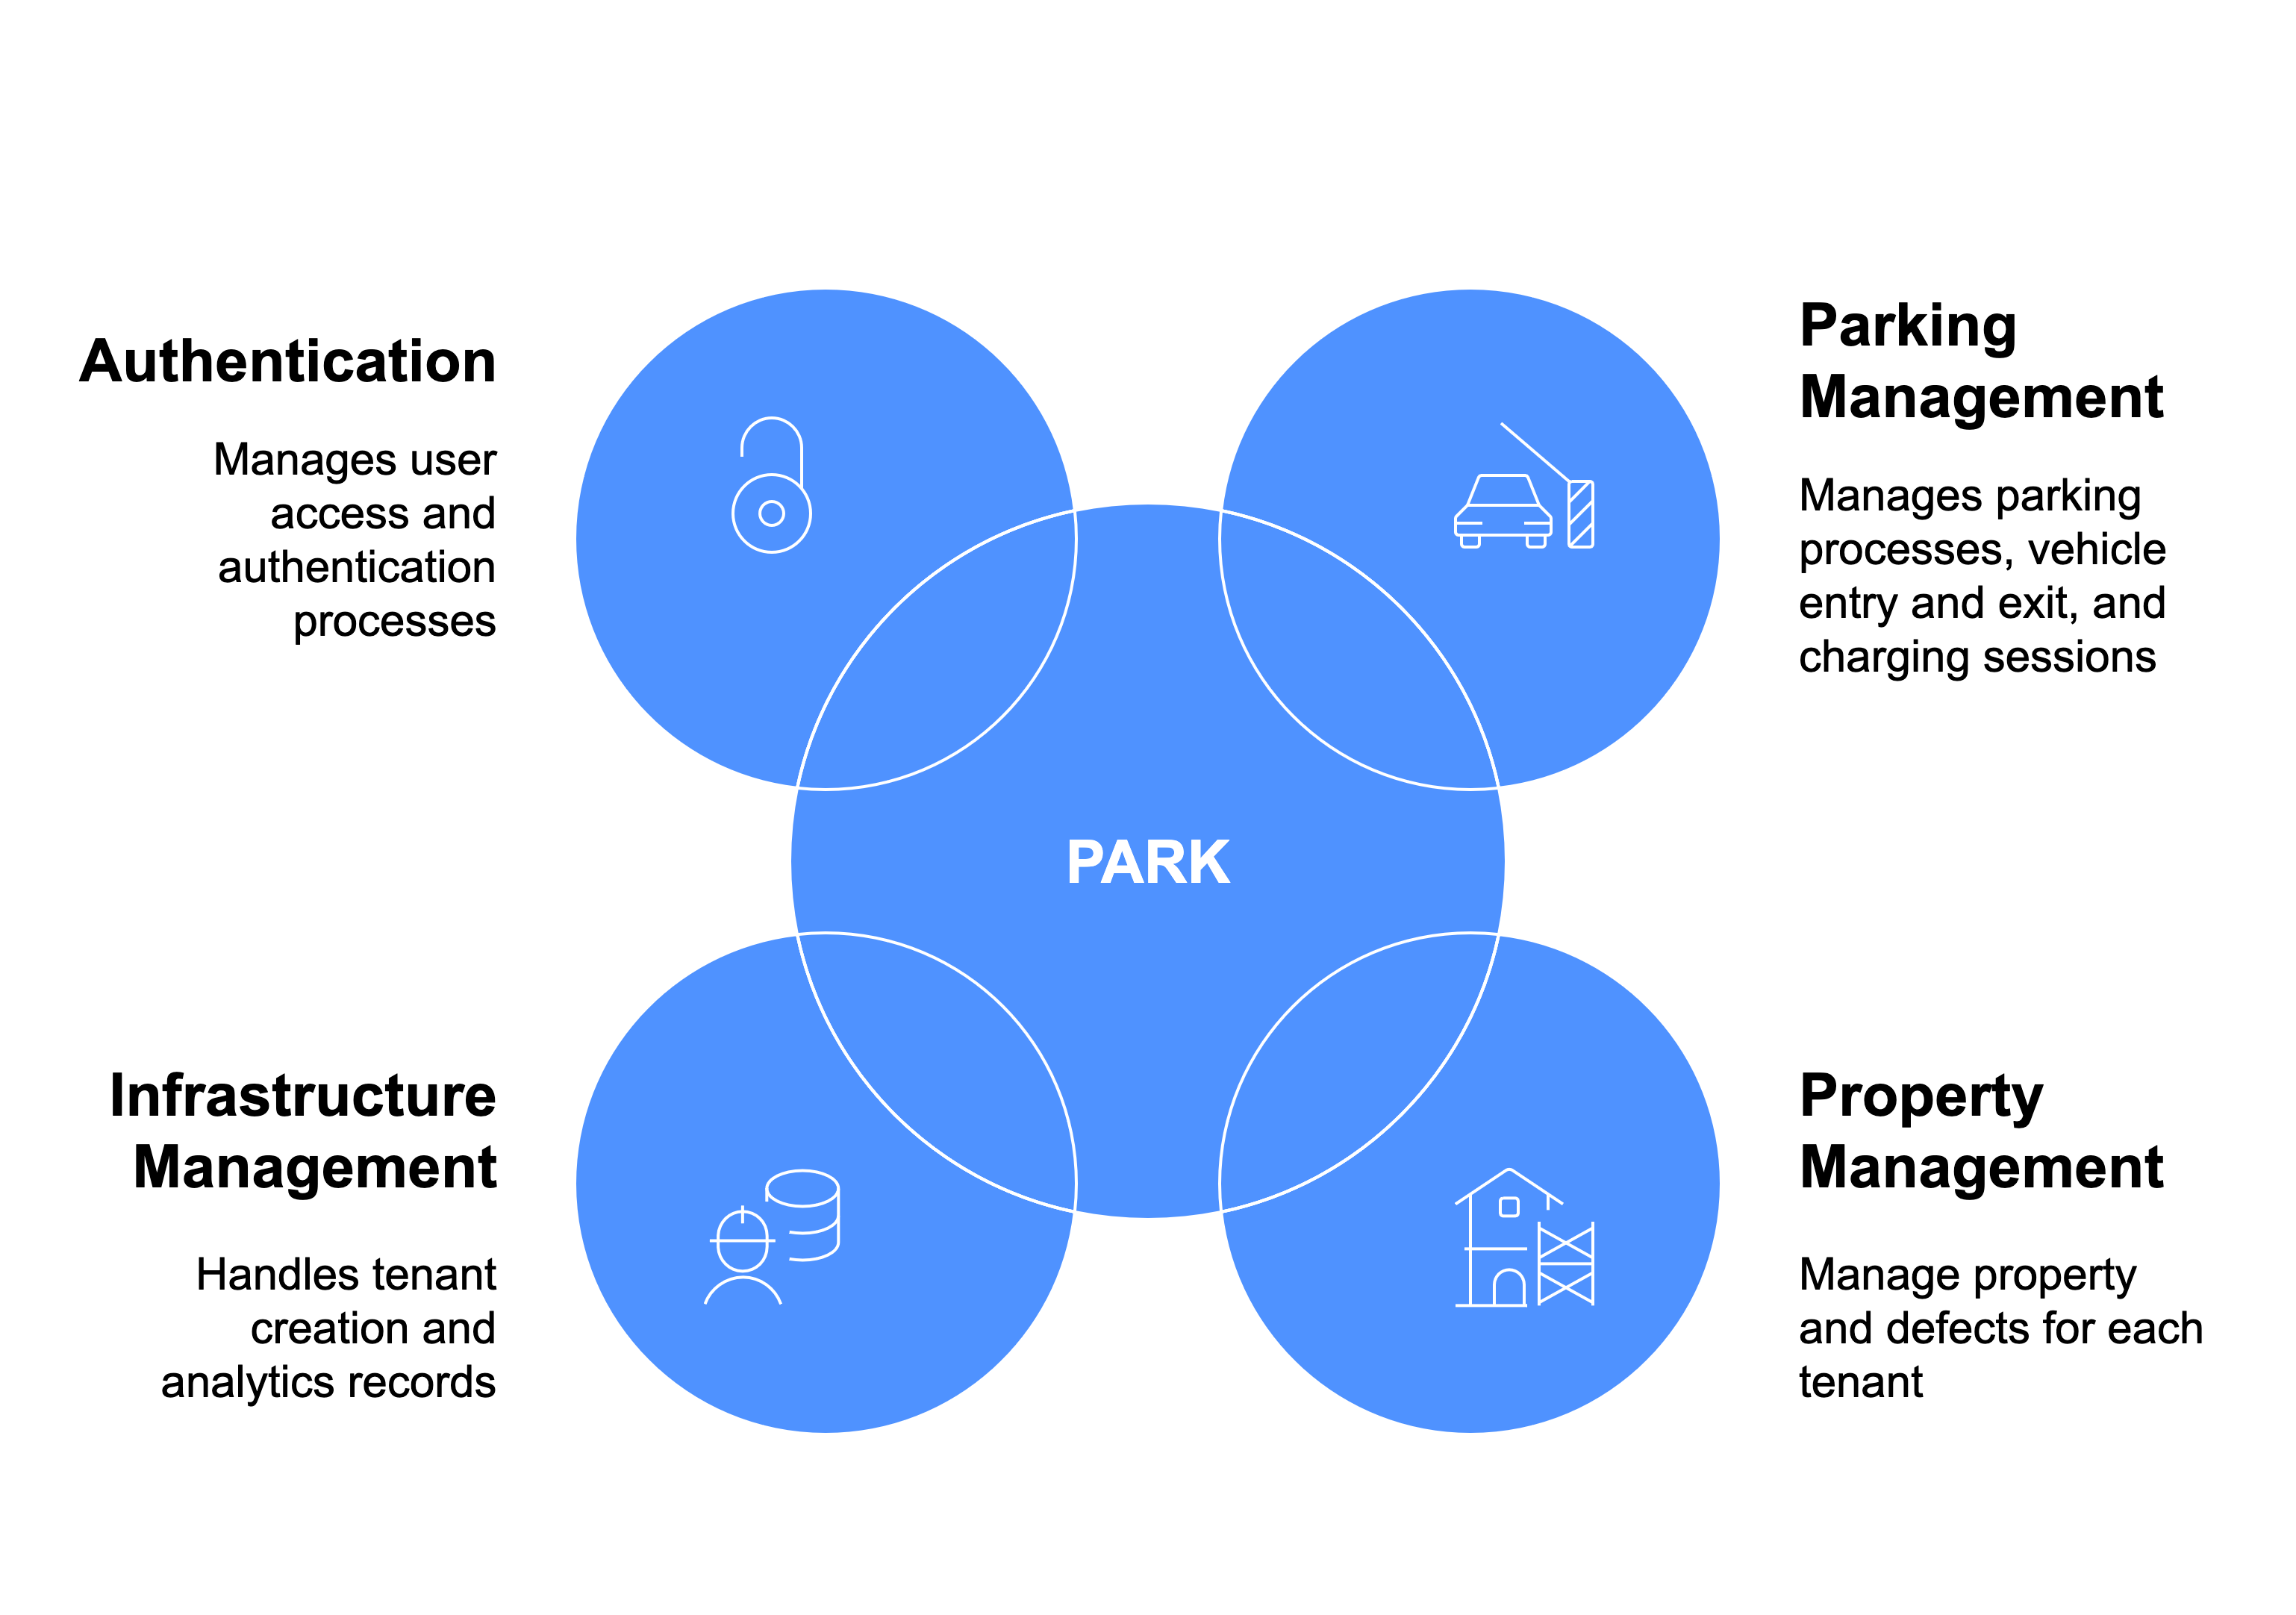
\includegraphics[width=0.9\textwidth]{resources/api-overview-blue.png}
    \caption{Übersicht der APIs}
    \label{fig:api-overview}
\end{figure}

Über die Parking Management API können alle Prozesse, die sich auf die Verwendung der Park- und Ladeinfrastruktur beziehen, verwendet werden. \\

\textbf{Parking Management:}
\begin{itemize}[noitemsep]
    \item[] \verb|GET garage/:garageId|
    \item[] \verb|POST garage/create|
    \item[] \verb|PUT garage/update|
    \item[] \verb|DELETE garage/delete/:garageId|
    \item[] \verb|GET garage/parking/occupancy/:garageId|
    \item[] \verb|GET garage/charging/occupancy/:garageId|
    \item[] \verb|POST garage/enter/:garageId|
    \item[] \verb|POST garage/handlePayment/:ticketId|
    \item[] \verb|GET garage/mayExit/:ticketId|
    \item[] \verb|POST garage/exit/:garageId|
    \item[] \verb|POST garage/charging/startSession/:garageId/:stationId/:userId|
    \item[] \verb|POST garage/charging/endSession/:garageId/:sessionId|
    \item[] \verb|GET garage/charging/session/:sessionId|
    \item[] \verb|GET garage/charging/invoice/:sessionId|
\end{itemize}

Die API des Property Management Services stellt alle Endpunkte für das Erstellen, Bearbeiten und Löschen der Parkhausinfrastruktur bereit. \\

\textbf{Property Management:}
\begin{itemize}[noitemsep]
    \item[] \verb|GET defects|
    \item[] \verb|GET defects/:id|
    \item[] \verb|POST defects|
    \item[] \verb|Put defects/:id|
    \item[] \verb|DELETE defects/:id|
    \item[] \verb|GET defects/signedUrl/:image|
    \item[] \verb|GET defects/signedUploadUrl/:image|
\end{itemize}

Im Infrastruktur Management Service ist die gesamte Analytics Funktionalität gebündelt. Für unterschiedliche Analysen können Records gespeichert werden (beispielsweise Belegung der Park- und Ladeplätze, Parkdauer, Energieverbrauch der Ladeinfrastruktur und Status der Defect-Verwaltung). Abgefragt werden können zumeist entweder die aktuellsten Werte für einen bestimmten Zeitpunkt oder eine Liste von Werten in einem bestimmten Zeitpunkt. Dieser Endpunkt wird beispielsweise für die Erstellung der Histogramme im Frontend verwendet. Der Aufbau dieser Records wird im folgenden Kapitel noch detaillierter beschrieben.
Neben den Analytics Endpunkten stellt der Service auch einen Endpunkt für die Erstellung eines neuen Tenants bereit. \\

\textbf{Infrastructure Management:}
\begin{itemize}[noitemsep]
    \item[] \verb|POST tenants/add|
    \item[] \verb|PUT analytics/parking/status/:tenantId/:garageId|
    \item[] \verb|GET analytics/parking/status/:garageId/:timestamp|
    \item[] \verb|GET analytics/parking/status/:garageId/:start/:end|
    \item[] \verb|PUT analytics/charging/status/:tenantId/:garageId|
    \item[] \verb|GET analytics/charging/status/:garageId/:timestamp|
    \item[] \verb|GET analytics/charging/status/:garageId/:start/:end|
    \item[] \verb|PUT analytics/parking/duration/:tenantId/:garageId/:duration|
    \item[] \verb|GET analytics/parking/duration/:garageId/:start/:end|
    \item[] \verb|PUT analytics/charging/powerConsumed/:tenantId/:garageId/:consumption|
    \item[] \verb|GET analytics/charging/powerConsumed/:garageId/:start/:end|
    \item[] \verb|PUT analytics/turnover/:tenantId/:garageId/:turnover|
    \item[] \verb|GET analytics/turnover/:garageId/:start/:end|
    \item[] \verb|PUT analytics/defects/status/:tenantId/:garageId|
    \item[] \verb|GET analytics/defects/status/:tenantId/:garageId/:timestamp|
    \item[] \verb|GET analytics/defects/status/:garageId/:start/:end|
    \item[] \verb|PUT analytics/requests/:tenantId|
    \item[] \verb|GET analytics/requests/:tenantId/:from/:to|
\end{itemize}

Die Schnittstelle des Authentication Service stellt einige Erweiterungen um die Google Cloud Identity Platform bereit, um beispielsweise Informationen über bestimmte Nutzer abzufragen. \\

\textbf{Authentication:}
\begin{itemize}[noitemsep]
    \item[] \verb|GET user/:userId|
    \item[] \verb|GET all-users|
    \item[] \verb|PUT user|
    \item[] \verb|POST user/:userId|
    \item[] \verb|DELETE user/:userId|
    \item[] \verb|POST tenants/add|
\end{itemize}

\subsection{Data Model}

In Abbildung \ref{fig:data-model} ist die Organisation der Daten dargestellt. Alle Objekte die für die Anwendung persistiert werden müssen, werden in Firestore gespeichert. Das betrifft beispielsweise User, Charging Sessions, Garagen, Tickets, usw. 

In den Figures \ref{fig:garage-object}, \ref{fig:analytics-record}, \ref{fig:charging-session-object}, \ref{fig:ticket-object}, \ref{fig:user-object} im Appendix sind die wichtigsten Objekte mit ihren Properties als JSON Objekte abgebildet.


Außerdem werden auch die Analytics Records in in Firestore gespeichert. Für die Analytics wird immer, wenn eine Änderung der entsprechenden Metrik verzeichnet wird ein neuer Record mit Zeitstempel abgespeichert, damit später in der Applikation der historische Verlauf für die Histogramme und rückblickende Analysen abgefragt werden kann. Für die Parking Status Analytics sieht ein solcher Analytics Record dann beispielsweise folgendermaßen aus:

\begin{verbatim}
    {
        "timestamp": "2025-01-23T15:10:55.391Z",
        "totalSpaces": 125,
        "occupiedSpaces": 98
    }
\end{verbatim}

Die Firestore Datenbanken für den Authentication Service und den Infrastructure-Management Service existieren einmal für die gesamte Anwendung, die Datenbanken für das Parking- und Property-Management existieren jeweils einmal für die Free-Tenants, einmal für die Premium-Tenants und für jeden Enterprise-Tenant. Gleich verhält es sich auch für die Collections, die mit dem Suffix \verb|-<tenantId>| versehen sind.

Neben den Firestore Datenbanken werden, wie in Abbildung \ref{fig:data-model} gezeigt, auch verschiedene Cloud Storage Buckets verwendet. Der Bucket \verb|gcf-source| beinhaltet dabei den Quellcode für die Cloud Function zur Erstellung der Defect Reports und wird für das Deployment benötigt. Die Defect Reports, die von dieser Cloud Function erstellt werden, werden wieder entsprechend des Tenants in einem Bucket abgelget (\verb|defect-reports-<tenantId>|). Der \verb|terraform-state| bucket wird ebenfalls für das Deployment benötigt, und umfasst neben den \verb|.tfstate| Files für Terraform auch zwei JSON Files für das Deployment und die Enterprise Tenants.
Darüber hinaus existiert noch ein Bucket \verb|prop-ma-<tenantId>|, in welchem die Bilder für die Defects abgespeichert werden können.

\begin{figure}[ht]
    \centering
    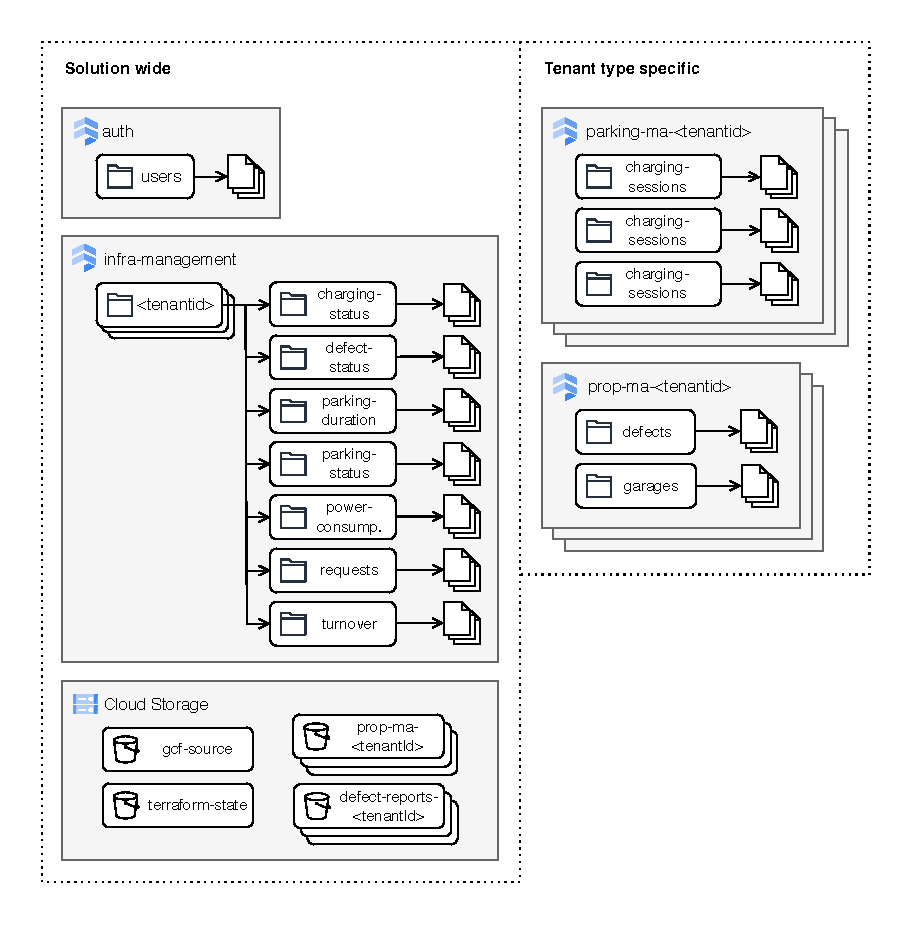
\includegraphics[width=\textwidth]{resources/data-model.drawio.pdf}
    \caption{Organisation der Daten in Firestore und Cloud Storage}
    \label{fig:data-model}
\end{figure}


\goodbreak
\section{Runtime View}
\subsection{Runtime Overview}

\begin{figure}[ht]
  \centering
  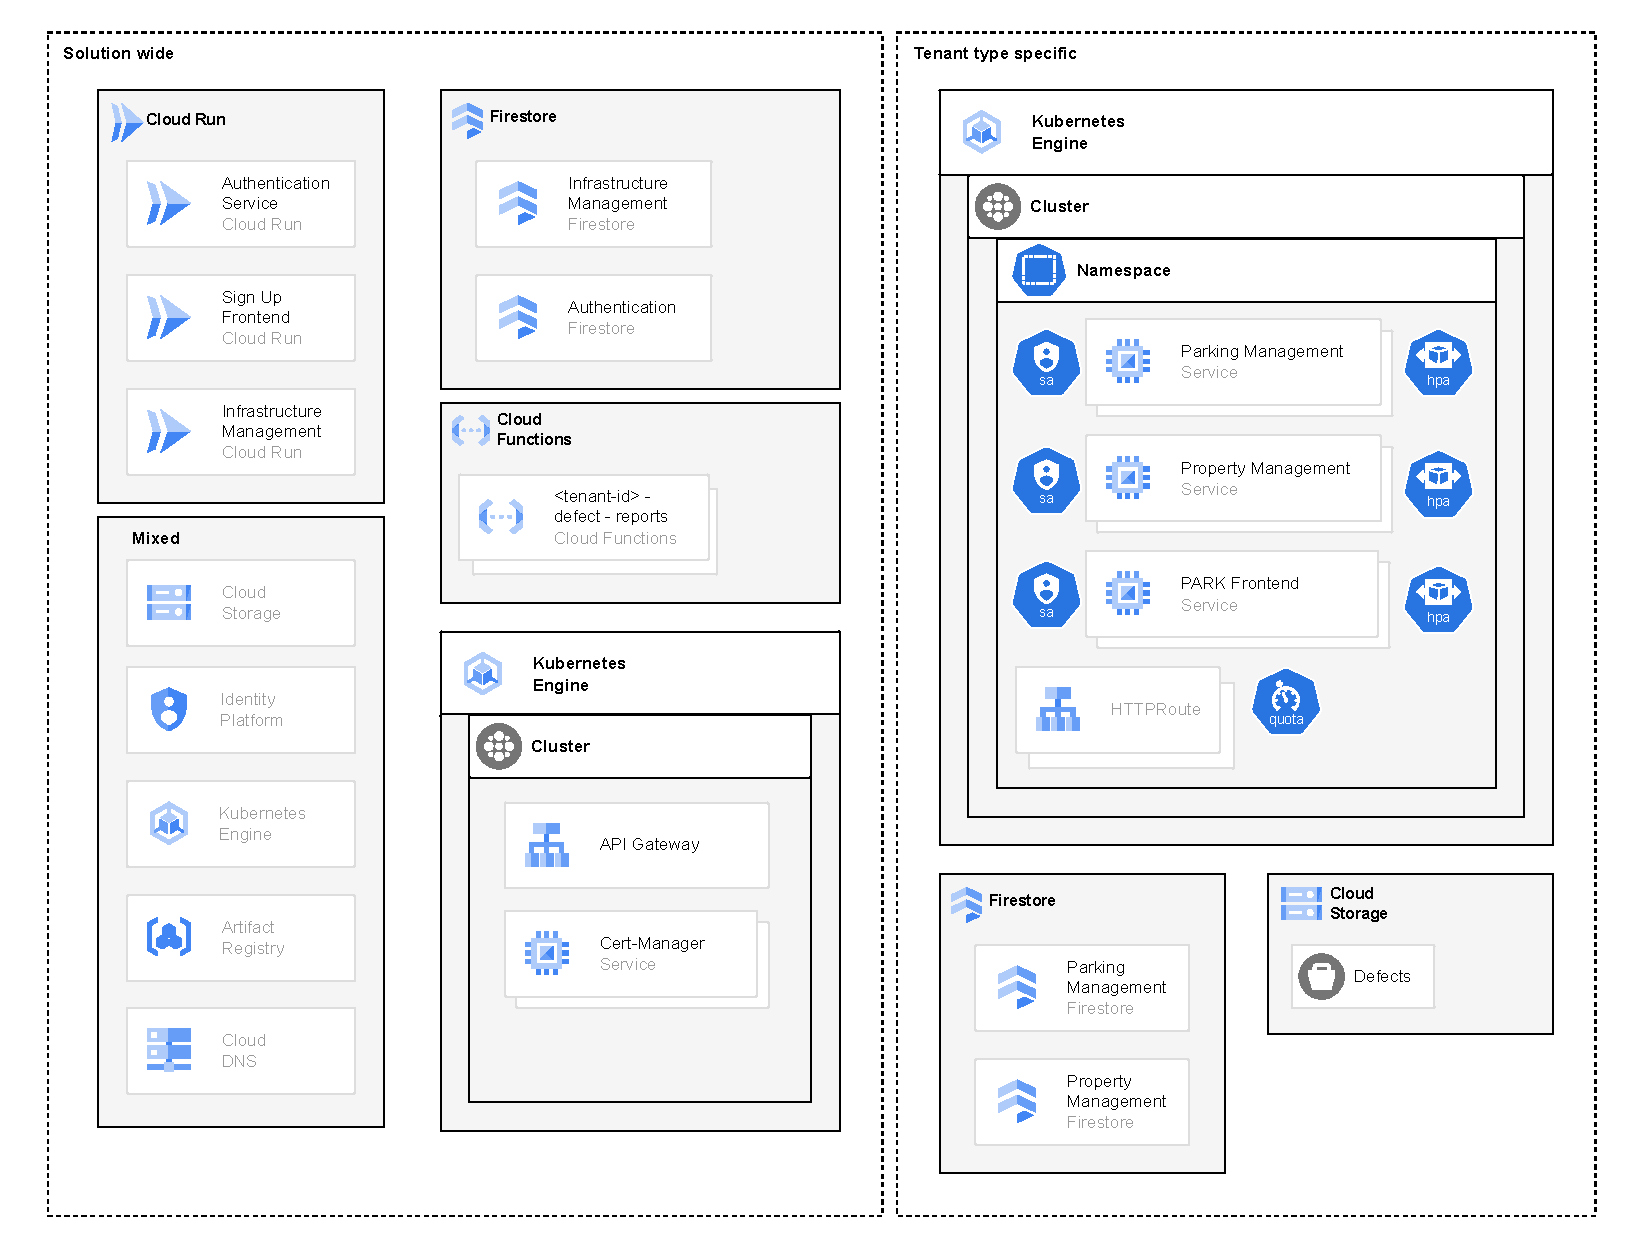
\includegraphics[width=\textwidth]{resources/03-runtime-view/pdf/cloud-ressources.pdf}
  \caption{Übersicht über die Cloud Ressourcen}
  \label{fig:cloud-ressources}
\end{figure}

\begin{figure}[ht]
  \centering
  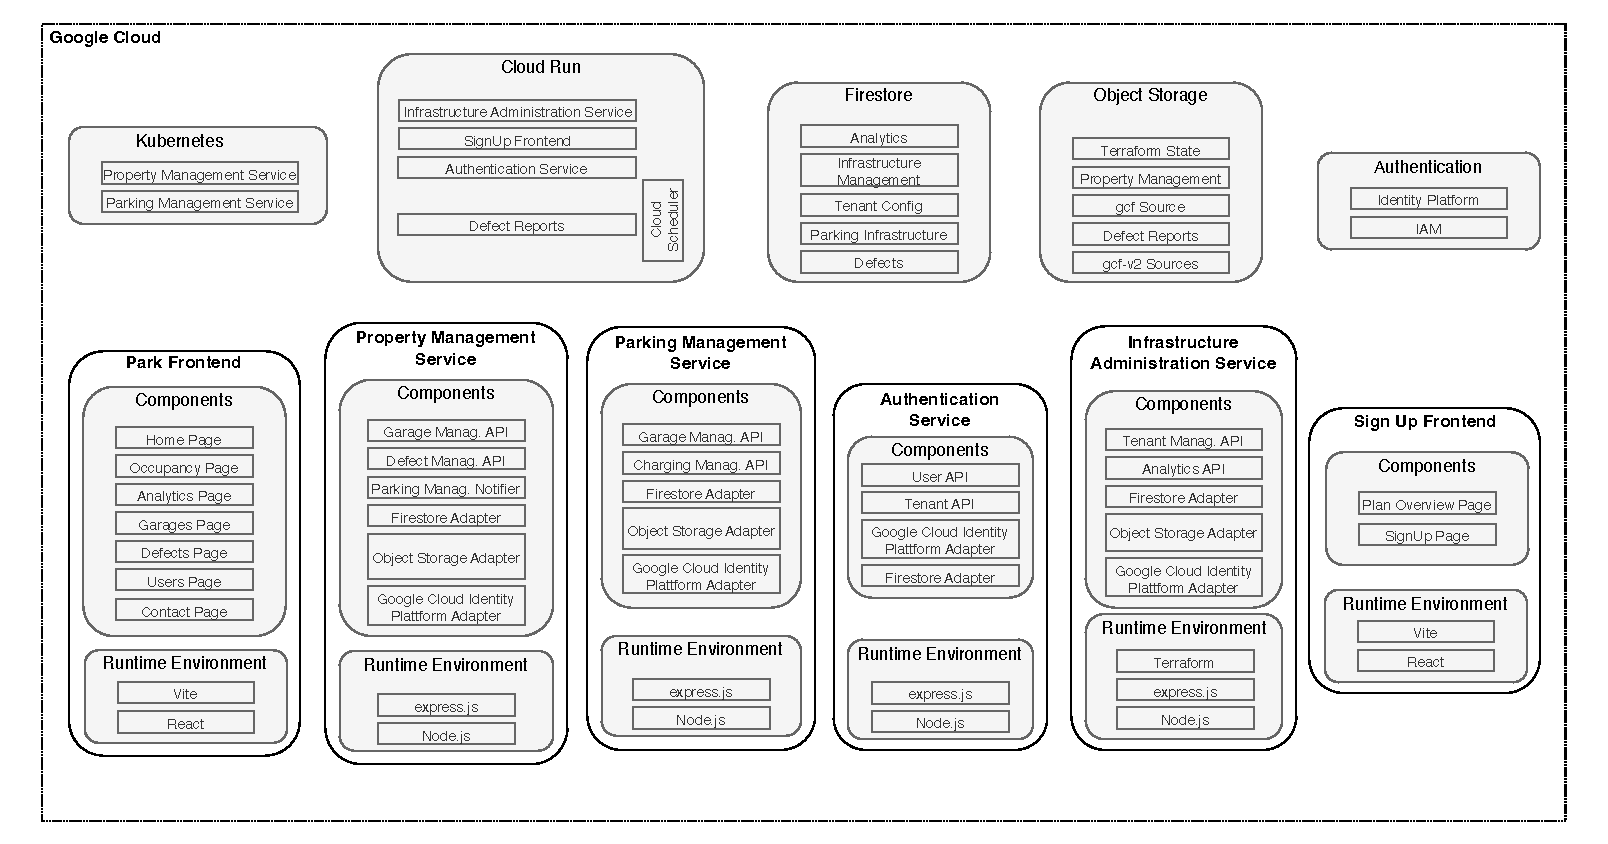
\includegraphics[width=\textwidth]{resources/03-runtime-view/pdf/architecture.pdf}
  \caption{Alle Mircoservices}
  \label{fig:system-architecture}
\end{figure}

In Abbildung~\ref{fig:cloud-ressources} werden alle verwendeten Cloud Ressourcen unterteilt in zwei Gruppen dargestellt:
\paragraph{Anwendungweite Ressources} sind Ressourcen, die von allen Tenants gemeinsam genutzt werden. 
Diese Ressourcen unterteilen sich nochmal in folgende Kategorien:
\begin{itemize}
  \item \textbf{Cloud Run} - Alle Services, welche in Cloud Run laufen. (Authentication Service, Infrastructure Management Service \& Sign Up Frontend)
  \item \textbf{Firestore} - Die Firestore Datenbanken, welche von den Cloud Run Services benötigt werden.
  \item \textbf{Cloud Functions} - Pro Tenant gibt es eine Defect-Report Cloud Function.
  \item \textbf{Mixed} - Weitere Cloud Ressourcen, welche für den Betrieb unsere Anwendung benötigt werden. (z.B. Cloud Storage, Identity Platform, Kubernetes Engine, Artifact Registry \& Ingres / DNS) 
\end{itemize}

\paragraph{Tenant Typ spezifische Ressources} sind Ressourcen, die sich von allen Tenants des selben Tenant Typs geteilt werden.
Jeder Enterprise Tenant wird hierbei als eigener Tenant Typ betrachtet, um die verwendeten Ressourcen bessere darstellen und erklären zu können. 
Die Ressourcen unterteilen sich nochmal in folgende Kategorien:
\begin{itemize}
  \item \textbf{Kubernetes} - Innerhalb der annwedungsweiten Kubernetes Engine existiert ein Cluster. Innerhalb des Cluster wird pro Tenant Typ ein neuer Namespace angelegt, in welchem die Services (Property Management \& Parking Management) laufen, welche sich alle Tenants eines Typs teilen.
  \item \textbf{Firestore} - Die Firestore Datenbanken, welche für die Services im Tenant Typ spezifischen Namespace benötigt werden. (Property Management \& Parking Management)
  \item \textbf{Cloud Storage} - Für den Property Management Service wird ein eigener Bucket angelegt, um die Bilder der Defects speichern zu können.
\end{itemize}

Um die Interaktionen zwischen den Komponenten als auch den anwendungweiten und Tenant Typ spezifischen Ressourcen zu verdeutlichen, wird in Abbildung~\ref{fig:system-architecture} die gesamte Systemarchitektur dargestellt. Hier sieht man, wie sich alle Komponenten eine Authentication Service und Infrastructure Management Service Instanz teilen.

\begin{figure}[ht]
  \centering
  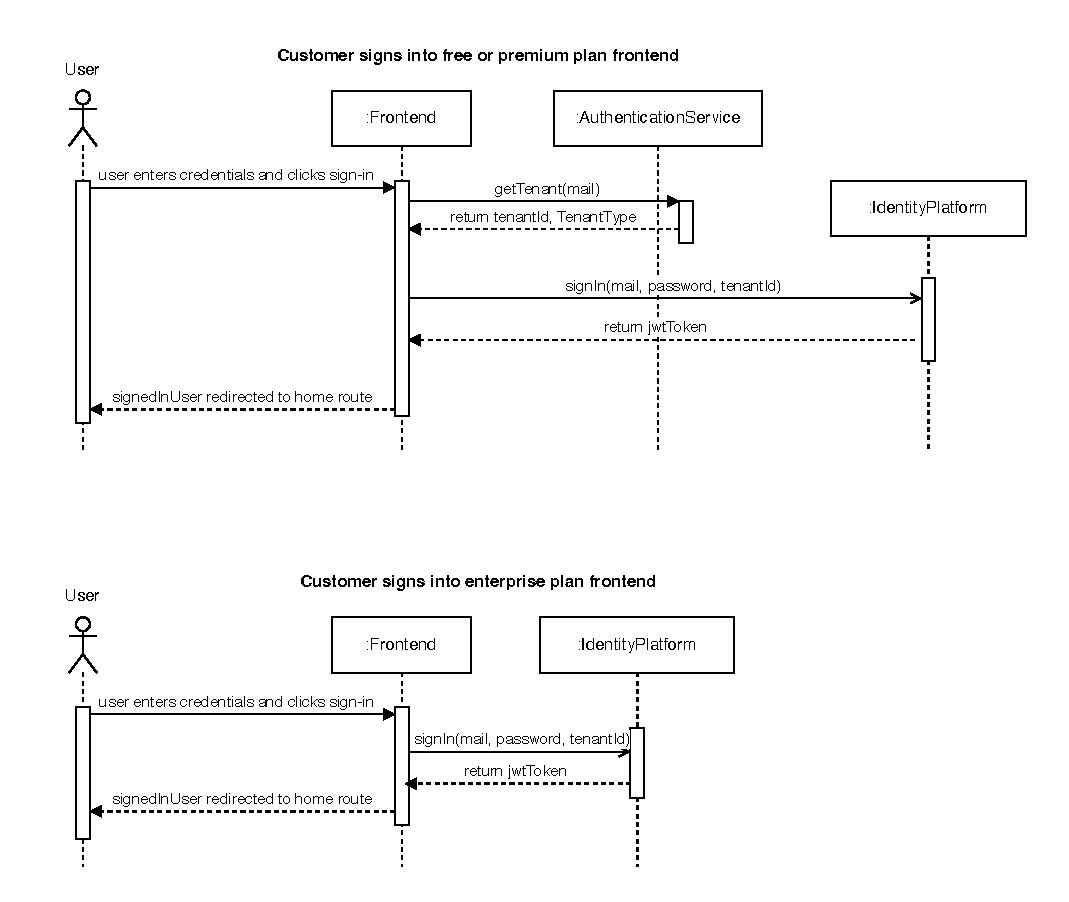
\includegraphics[width=\textwidth]{resources/03-runtime-view/pdf/authentication-sequence.pdf}
  \caption{Ablauf der Tenant Typ abhängigen Authentifizierung}
  \label{fig:authentication-sequence}
\end{figure}

Eine Besonderheit ist hierbei die Authentifizierung mittels Authentication Service und Identity Platform. In Abbildung~\ref{fig:authentication-sequence} wird der Ablauf der Authentifizierung dargestellt. Das heißt wenn sich ein Nutzer in seiner Tenant Typ spezifischen Instanz des Frontends anmeldet, wird zuerst über den Authentication Service abgefragt, ob der Nutzer überhaupt vom richtigen Tenant Typ ist und falls ja die Tenant Id, zu welchem der Nutzer gehört. Anschließend wird der Nutzer Tenant-Aware über die Identity Platform authentifiziert. Wenn die Authentifizierung erfolgreich war, wird der Nutzer auf die entsprechende Home-Seite weitergeleitet und im Hintergrund im Local-Storage ein JWT Token zu Authentifizierung im Backend abgelegt. 
Für den Tenant Typ Enterprise entfällt die Anfrage an den Authentication Service, da diese Frontend nur von einem Tenant verwendet wird und daher die Tenant Id als Konstante im Environment hinterlegt ist.

\begin{figure}[ht]
  \centering
  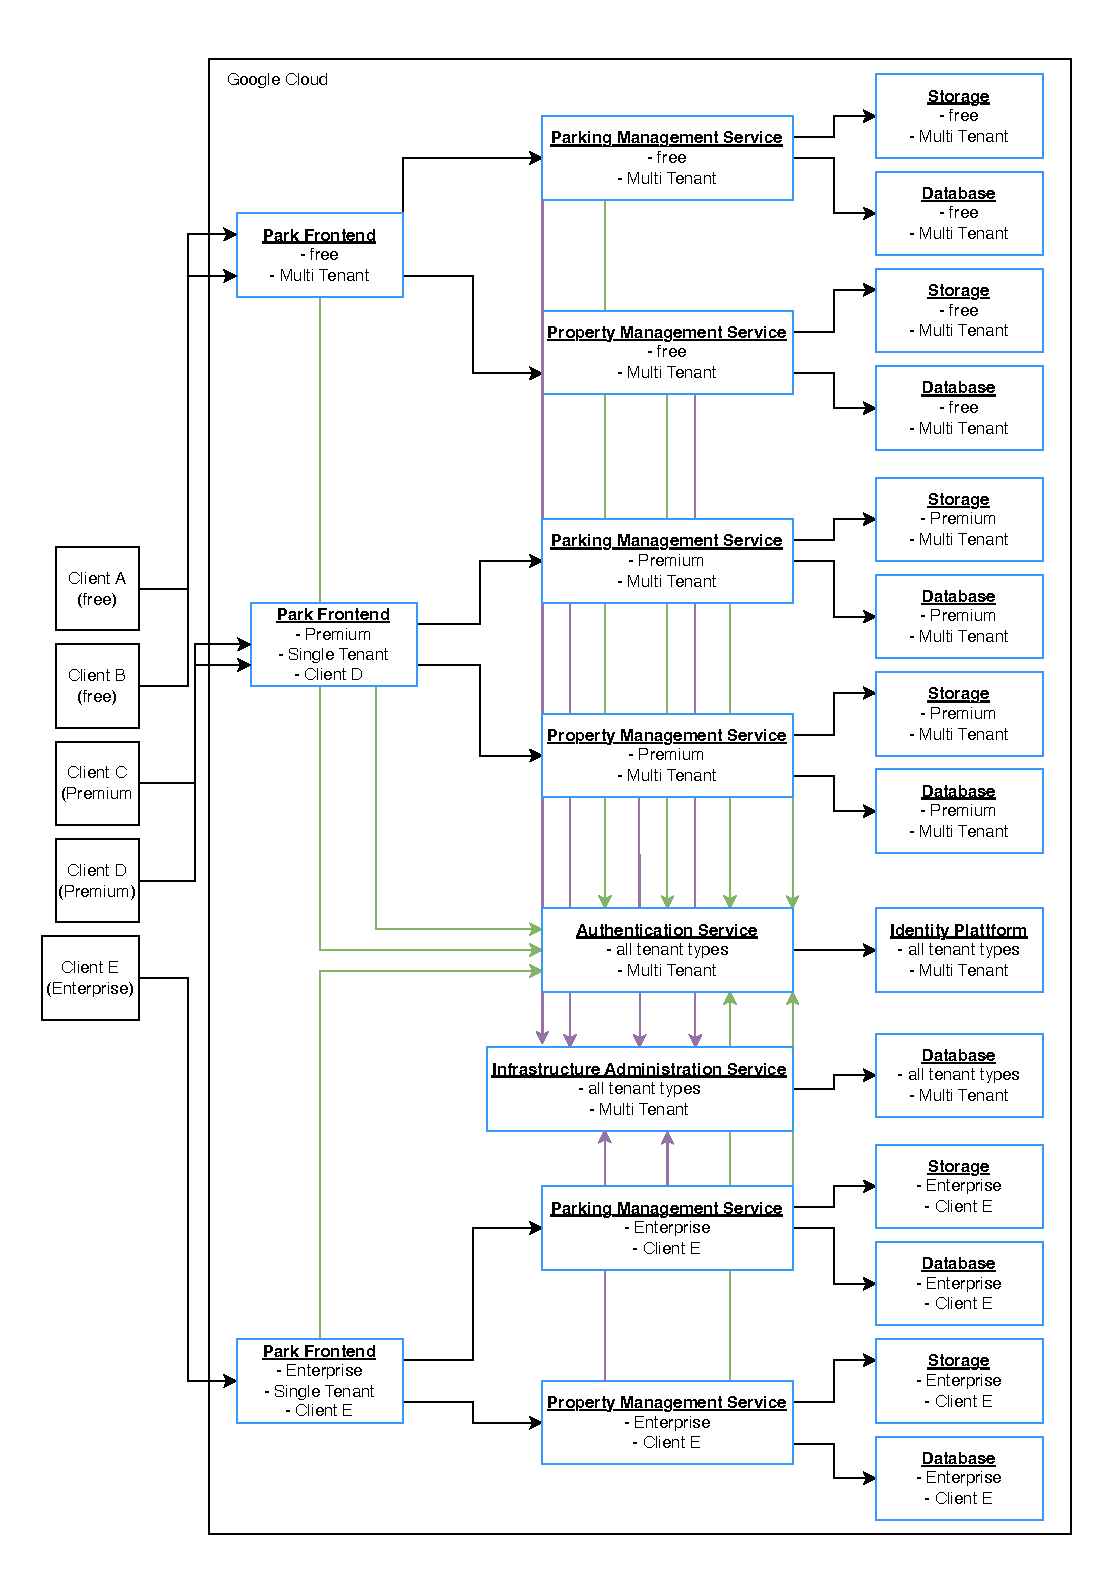
\includegraphics[width=0.95\textwidth]{resources/03-runtime-view/pdf/components-frontend-park.pdf}
  \caption{Alle verwendeten Komponenten, wenn ein Client mit dem Park Frontend interagiert, mit Berücksichtigung von Multitenancy}
  \label{fig:components-park-frontend}
\end{figure}

\begin{figure}[ht]
  \centering
  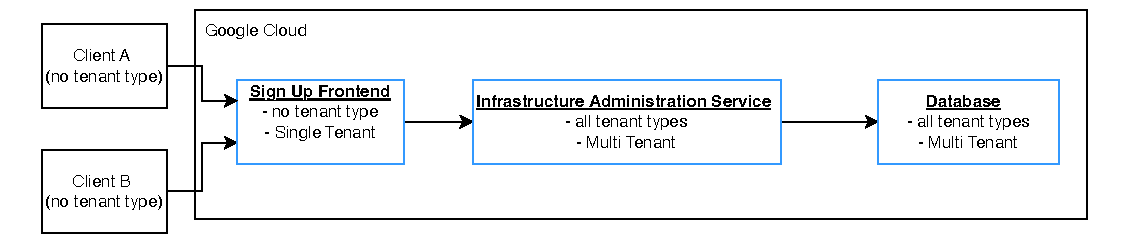
\includegraphics[width=\textwidth]{resources/03-runtime-view/pdf/components-frontend-signup.pdf}
  \caption{Alle verwendeten Komponenten, wenn ein Client mit dem Signup Frontend interagiert}
  \label{fig:components-signup-frontend}
\end{figure}

\subsection{Mircoservices}

{\rowcolors{2}{}{gray!20}
\begin{longtable}{l p{6cm}}
  \caption{Environment-Variablen für den Authentication Service}
  \label{tab:auth-service-env-vars} \\
  \textbf{Environment-Variable} & \textbf{Beschreibung} \\ [1ex]
  \texttt{IDENTITY\_PLATFORM\_API\_KEY} & API-Schlüssel für die Identity Platform \\ [0.5ex]
  \texttt{IDENTITY\_PLATFORM\_AUTH\_DOMAIN} & Authentifizierungs-Domain für die Identity Platform \\ [0.5ex]
  \texttt{IDENTITY\_PLATFORM\_PROJECT\_ID} & Projekt-ID der Identity Platform \\ [0.5ex]
  \texttt{FIRESTORE\_DB\_ID} & Identifier für die Firestore-Datenbank \\ [0.5ex]
  \texttt{PORT} & Port, auf dem der Service läuft \\ [0.5ex]
  \texttt{INFRASTRUCTURE\_SERVICE\_URL} & URL für den Infrastructure Service \\ [0.5ex]
  \texttt{INFRASTRUCTURE\_ADMINISTRATION\_SERVICE\_AUDIENCE} & Zielgruppe des Administration Service \\ 
\end{longtable}}


% Infrastructure Administration Service Table
{\rowcolors{2}{}{gray!20}
\begin{longtable}{l p{6cm}}
  \caption{Environment-Variablen für den Infrastructure Administration Service}
  \label{tab:infra-admin-service-env-vars} \\
  \textbf{Environment-Variable} & \textbf{Beschreibung} \\ [1ex]
  \texttt{AUTHENTICATION\_SERVICE\_URL} & URL des Authentication Service \\ [0.5ex]
  \texttt{ANALYTICS\_DB\_ID} & Identifier für die Analytics-Datenbank \\ [0.5ex]
  \texttt{INFRASTRUCTURE\_ADMINISTRATION\_SERVICE\_AUDIENCE} & Zielgruppe des Administration Service \\ [0.5ex]
  \texttt{PORT} & Port, auf dem der Service läuft \\ [0.5ex]
  \texttt{GITHUB\_ACTION\_TOKEN} & Token für GitHub-Aktionen \\ [0.5ex]
  \texttt{GITHUB\_TENANT\_WORKFLOW\_ID} & ID des GitHub-Tenant-Workflows \\ [0.5ex]
  \texttt{GITHUB\_TENANT\_WORKFLOW\_BRANCH} & Branch für den GitHub-Tenant-Workflow \\ 
\end{longtable}}

% Parking Management Service Table
{\rowcolors{2}{}{gray!20}
\begin{longtable}{l p{6cm}}
  \caption{Environment-Variablen für den Parking Management Service}
  \label{tab:parking-mgmt-service-env-vars} \\
  \textbf{Environment-Variable} & \textbf{Beschreibung} \\ [1ex]
  \texttt{FIRESTORE\_DB\_ID} & Identifier für die Firestore-Datenbank \\ [0.5ex]
  \texttt{AUTHENTICATION\_SERVICE\_URL} & URL des Authentication Service \\ [0.5ex]
  \texttt{INFRASTRUCTURE\_MANAGEMENT\_SERVICE\_URL} & URL des Infrastructure Management Service \\ [0.5ex]
  \texttt{INFRASTRUCTURE\_ADMINISTRATION\_SERVICE\_AUDIENCE} & Zielgruppe des Administration Service \\ [0.5ex]
  \texttt{PORT} & Port, auf dem der Service läuft \\ 
\end{longtable}}

% Property Management Service Table
{\rowcolors{2}{}{gray!20}
\begin{longtable}{l p{6cm}}
  \caption{Environment-Variablen für den Property Management Service}
  \label{tab:property-mgmt-service-env-vars} \\
  \textbf{Environment-Variable} & \textbf{Beschreibung} \\ [1ex]
  \texttt{FIRESTORE\_DB\_ID} & Identifier für die Firestore-Datenbank \\ [0.5ex]
  \texttt{GCS\_BUCKET\_ID} & Identifier für den Google Cloud Storage Bucket \\ [0.5ex]
  \texttt{PARKING\_MANAGEMENT\_BACKEND\_URL} & URL des Parking Management Backends \\ [0.5ex]
  \texttt{AUTHENTICATION\_SERVICE\_URL} & URL des Authentication Service \\ [0.5ex]
  \texttt{INFRASTRUCTURE\_MANAGEMENT\_SERVICE\_URL} & URL des Infrastructure Management Service \\ [0.5ex]
  \texttt{INFRASTRUCTURE\_ADMINISTRATION\_SERVICE\_AUDIENCE} & Zielgruppe des Administration Service \\ [0.5ex]
  \texttt{PORT} & Port, auf dem der Service läuft \\ 
\end{longtable}}

% Park Frontend Table
{\rowcolors{2}{}{gray!20}
\begin{longtable}{l p{6cm}}
  \caption{Environment-Variablen für das Park Frontend}
  \label{tab:park-frontend-env-vars} \\
  \textbf{Environment-Variable} & \textbf{Beschreibung} \\ [1ex]
  \texttt{VITE\_TENANT\_ID} & ID des Tenants \\ [0.5ex]
  \texttt{VITE\_TENANT\_TYPE} & Typ des Tenants \\ [0.5ex]
  \texttt{VITE\_PROPERTY\_MANAGEMENT\_SERVICE\_URL} & URL des Property Management Services \\ [0.5ex]
  \texttt{VITE\_AUTHENTICATION\_SERVICE\_URL} & URL des Authentication Services \\ [0.5ex]
  \texttt{VITE\_PARKING\_MANAGEMENT\_SERVICE\_URL} & URL des Parking Management Services \\ [0.5ex]
  \texttt{VITE\_INFRASTRUCTURE\_MANAGEMENT\_SERVICE\_URL} & URL des Infrastructure Management Services \\ [0.5ex]
  \texttt{VITE\_IDENTITY\_PLATFORM\_API\_KEY} & API-Schlüssel für die Identity Platform \\ [0.5ex]
  \texttt{VITE\_IDENTITY\_PLATFORM\_AUTH\_DOMAIN} & Authentifizierungs-Domain für die Identity Platform \\ [0.5ex]
  \texttt{VITE\_IDENTITY\_PLATFORM\_PROJECT\_ID} & Projekt-ID der Identity Platform \\ 
\end{longtable}}

% Sign Up Frontend Table
{\rowcolors{2}{}{gray!20}
\begin{longtable}{l p{6cm}}
  \caption{Environment-Variablen für das Sign Up Frontend}
  \label{tab:signup-frontend-env-vars} \\
  \textbf{Environment-Variable} & \textbf{Beschreibung} \\ [1ex]
  \texttt{VITE\_AUTHENTICATION\_SERVICE\_URL} & URL des Authentication Services \\ 
\end{longtable}}

In Abbildung~\ref{fig:components-park-frontend} und Abbildung~\ref{fig:components-signup-frontend} werden alle Komponenten dargestellt, welche bei einer Interaktion mit dem Park Frontend oder dem Sign Up Frontend verwendet werden.
% TODO: Runtime Konfiguration
% TODO: Scaling
% TODO: Customization
% TODO: Security Setup
% TODO: Vbd. zu Datenbanken
\subsection{Data Stores}
\goodbreak
\section{DevOps}

Im Folgenden werden alle Aspekte des DevOps-Prozesses beschrieben, 
die für die Entwicklung und den Betrieb der Anwendung relevant sind. 
Dies beinhaltet die Bereitstellung von Umgebungen, Rollen und Serviceaccounts, 
Pipelines und die Veröffentlichung neuer Features, die Einrichtung neuer Tenants, 
das Monitoring und das Load Testing.

\subsection{Umgebungen / Environments}

Für die Entwicklung und den Betrieb der Anwendung werden verschiedene Umgebungen (Environments) verwendet.
Für den Betrieb der Anwendung wird die \glqq{}Production\grqq{}-Umgebung verwendet, für 
die Entwicklung wird die \glqq{}Staging\grqq{}-Umgebung verwendet. 
Eine weitere \glqq{}Development\grqq{}-Umgebung wurde aufgrund der geringen Anzahl an Entwicklern 
nicht eingerichtet. Werden für die lokale Entwicklung Cloud-Dienste wie Firestore oder 
Storage Buckets benötigt, werden der Einfachheit halber diese aus der \glqq{}Staging\grqq{}-Umgebung 
verwendet.

Jede Umgebung wird in einem eigenen Projekt in der Google Cloud Platform betrieben.
So wird eine klare Trennung zwischen den Umgebungen gewährleistet.
Da beide Umgebungen über IAC (Infrastructure as Code) verwaltet werden,
sind die Umgebungen identisch und können außerdem schnell wiederhergestellt werden.

\subsubsection{Ressourcen pro Umgebung}

Tabelle \ref{tab:google-cloud-ressourcen} listet die Google Cloud Ressourcen pro Umgebung auf und
beschreibt kurz deren Funktion. Da die Umgebungen identisch sind, ist nur eine Tabelle notwendig.

\renewcommand{\arraystretch}{1.5}
{\rowcolors{2}{}{gray!20}
\begin{longtable}{l p{10cm}}
  \caption{Google Cloud Ressourcen pro Umgebung}
  \label{tab:google-cloud-ressourcen} \\
  \textbf{Ressource} & \textbf{Beschreibung} \\ [1ex]
  Kubernetes Cluster & Cluster, auf dem die Anwendung läuft. \\ [0.5ex]
  Storage Buckets  & Storage Buckets zur Speicherung von Defect Bildern, Defect Reports und anderen Dateien wie z.B. den Terraform State Files. \\ [0.5ex]
  Firestore & Firestore Datenbank zur Speicherung von Daten. \\ [0.5ex]
  Identity Platform & Identity Platform zur Verwaltung von Benutzern und Tenants \\ [0.5ex]
  Identity Federation & Identity Federation zur Authentifizierung von GitHub ohne Credentials. \\ [0.5ex]
  Cloud Run & Cloud Run für Services, die nicht im Kubernetes Cluster laufen. \\ [0.5ex]
  Artifact Registry & Ein Repository für Docker Images in der Artifact Registry \\ [0.5ex]
  DNS Zone & DNS Zone zur Verwaltung der Subdomains der einzelnen Tenants. \\ [0.5ex]
\end{longtable}}

\subsubsection{Tenant Isolation}

Die Isolation der Tenants im Kubernetes Cluster wird durch die Verwendung von Namespaces erreicht.
Es gibt einen Namespace für die \textit{free} Tenants und einen für die \textit{premium} Tenants.
Die Tenants in den \textit{free} bzw. \textit{premium} Namespaces teilen sich die dem Namespace zugewiesenen Ressourcen.
Enterprise Tenants erhalten einen eigenen Namespace. 
Die darin enthaltenen Ressourcen sind nur für diesen Tenant verfügbar.

Die Isolation der Tenants in der Google Cloud Platform wird durch die Verwendung von 
separaten Buckets und Firestore Datenbanken erreicht. Die Ressourcen werden dabei 
analog zu den Kubernetes Namespaces aufgeteilt. Die \textit{free} und \textit{premium} Tenants
teilen sich die Ressourcen wie Buckets und Firestore Datenbanken. Die Enterprise Tenants
erhalten eigene Ressourcen.

Für die Isolation innerhalb der geteilten Ressourcen, werden in den Buckets Unterordner und in 
den Firestore Datenbanken separate Collections für die Tenants angelegt.

\subsection{Roles and Role Mapping}

Da das Team aus nur drei Mitgliedern besteht, wurde auf eine detaillierte Aufteilung der Rollen unter
den Teammitgliedern verzichtet. Jedes Teammitglied hat Zugriff auf alle Ressourcen in dem jeweiligen Projekt.
Dafür wurde jedem Teammitglied die Rolle \textit{roles/owner} zugewiesen.

\subsubsection{Dienstkonten}

Um die einzelnen Services der Park Anwendung zu authentifizieren, wurde pro Service ein Dienstkonto erstellt.
Genauer wurde pro Service pro Namespace ein Dienstkonto angelegt weil ein Service aus dem \textit{free}
Namespace nicht auf die Ressourcen eines Services aus dem \textit{premium} Namespace zugreifen darf.

Um keine Credentials in den Services speichern zu müssen, 
wurde die \glqq{}Workload Identity Federation for GKE\grqq{}\footnote{https://cloud.google.com/kubernetes-engine/docs/concepts/workload-identity} verwendet.
Diese muss bei der Erstellung des Clusters aktiviert werden und läuft auf den Nodes des Clusters. 
Die Workload Identity Federation unterscheidet zwischen Dienstkonten 
der Google Cloud Platform und Dienstkonten des Kubernetes Clusters.

\begin{itemize}
  \item \textbf{Kubernetes-Dienstkonten} sind Kubernetes-Ressourcen, die eine Identität für Prozesse bereitstellen, 
  die in Ihren GKE-Pods ausgeführt werden.
  \item \textbf{IAM-Dienstkonten} sind Google Cloud-Ressourcen, 
  mit denen Anwendungen autorisierte Aufrufe an Google Cloud APIs ausführen können.
\end{itemize}

Die Workload Identity Federation ermöglicht es, dass ein Kubernetes-Dienstkonto auf ein IAM-Dienstkonto gemappt wird.
Damit das Mapping funktioniert, muss das Kubernetes-Dienstkonto in der Annotation 
\textit{iam.gke.io/gcp-service-account} die E-Mail-Adresse des IAM-Dienstkontos enthalten.
\footnote{https://cloud.google.com/kubernetes-engine/docs/how-to/workload-identity\#kubernetes-sa-to-iam}


Um den Zugriff auf die Google Cloud Ressourcen aus GitHub Actions zu ermöglichen,
wurde pro Projekt ein weiteres Dienstkonto erstellt. Dieses Dienstkonto hat nur die minimalen Rechte,
die für die Ausführung der GitHub Actions notwendig sind. Durch die \glqq{}Workload Identity Federation\grqq{}
(das ist eine andere Workload Identity Federation als die für GKE) müssen keine Credentials
in den GitHub Secrets gespeichert werden.\footnote{https://cloud.google.com/blog/products/identity-security/enabling-keyless-authentication-from-github-actions?hl=en}

\subsection{Pipelines and Release of new Features}

Für die Bereitstellung von neuen Features und Bugfixes wird ein CI/CD-Prozess verwendet.
Die CI/CD-Pipeline wird mit GitHub Actions realisiert.
Die gesamte Pipeline ist in mehrere Actions unterteilt, wobei die eine Action bei Pull-Requests ausgeführt wird,
die andere bei einem Push auf den \textit{dev}- oder \textit{main}-Branch.

\subsubsection*{Pipeline für Pull-Requests auf \textit{dev} und \textit{main}}

Die Pipeline für Pull-Requests besteht aus den folgenden Jobs:
\begin{itemize}
  \item \textbf{Build}: Die Docker Images aller Services werden gebaut und auf eventuelle Fehler überprüft.
  \item \textbf{Test}: Die Unittests der Services werden ausgeführt.
  \item \textbf{Plan Terraform for the Infrastructure}: Die Änderungen an der Infrastruktur werden geplant.
  \item \textbf{Plan Terraform for the Application}: Die Änderungen an der Anwendung werden geplant.
\end{itemize}

Je nachdem, ob es sich um einen Push auf den \textit{dev}- oder \textit{main}-Branch handelt, wird die Pipeline
für die \textit{staging}- oder \textit{production}-Umgebung ausgeführt. 
Abbildung \ref{fig:pr-pipeline} zeigt die Pipeline für Pull-Requests.

\begin{figure}[ht]
  \centering
  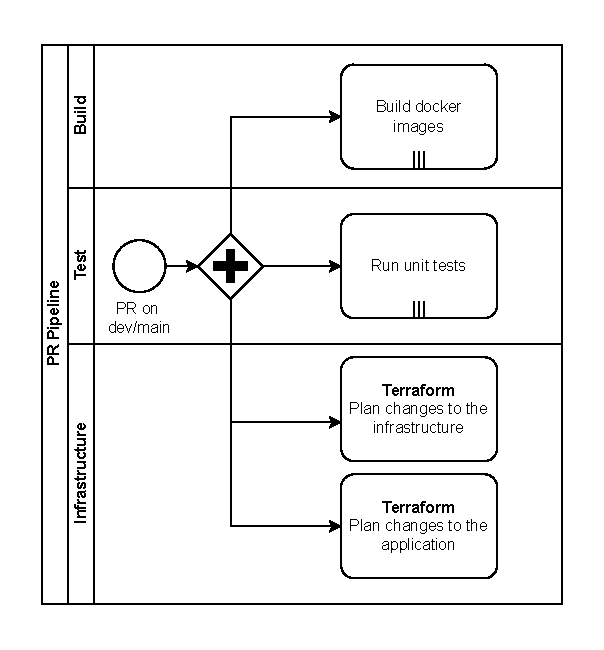
\includegraphics[width=0.6\textwidth]{resources/pr-pipeline.pdf}
  \caption{PR Pipeline}
  \label{fig:pr-pipeline}
\end{figure}


\subsubsection*{Pipeline für Push auf \textit{dev} und \textit{main}}

Die Pipeline für einen Push auf den \textit{dev}- oder \textit{main}-Branch ist für das 
Deployment der Änderungen in der Infrastruktur und der Anwendung zuständig.
Die Pipeline besteht aus den folgenden Jobs:

\begin{itemize}
  \item \textbf{Apply Terraform for the Infrastructure}: Die Änderungen an der Infrastruktur werden angewendet.
  \item \textbf{Build and Push Images}: Die Docker Images aller Services werden gebaut und in die Artifact Registry hochgeladen.
  \item \textbf{Package Cloud Functions}: Die Cloud-Functions werden in ein Zip-Archiv gepackt.
  \item \textbf{Apply Terraform for the Application}: Die Änderungen an der Anwendung werden angewendet. Das beinhaltet das Deployment der Docker Images und der Cloud-Functions.
  \item \textbf{Deploy Cloud Run}: Cloud-Run-Services, die nicht im Kubernetes Cluster laufen, werden deployed.
  \item \textbf{Update deployment.json}: Deployment-Informationen wie der Tag der Images werden in einer JSON-Datei in einem Bucket für spätere Pipelines gespeichert.
\end{itemize}

Da die Park Anwendung Multi-Tenant-fähig ist, müssen die Tenants auch in den Pipelines berücksichtigt werden.
Viele Ressourcen wie Buckets, Firestore Datenbanken und DNS-Zonen müssen pro Enterprise Tenant erstellt werden.
Um herauszufinden, ob Ressourcen erstellt, aktualisiert oder gelöscht werden müssen, wird eine JSON-Datei 
aus einem Bucket geladen. Diese Datei enthält die Konfiguration der Enterprise Tenants.

Je nachdem, ob es sich um einen Push auf den \textit{dev}- oder \textit{main}-Branch handelt, wird die Pipeline
für die \textit{staging}- oder \textit{production}-Umgebung ausgeführt.
Abbildung \ref{fig:cd-pipeline} zeigt die Pipeline für einen Push auf den \textit{dev}- oder \textit{main}-Branch.

\begin{figure}[ht]
  \centering
  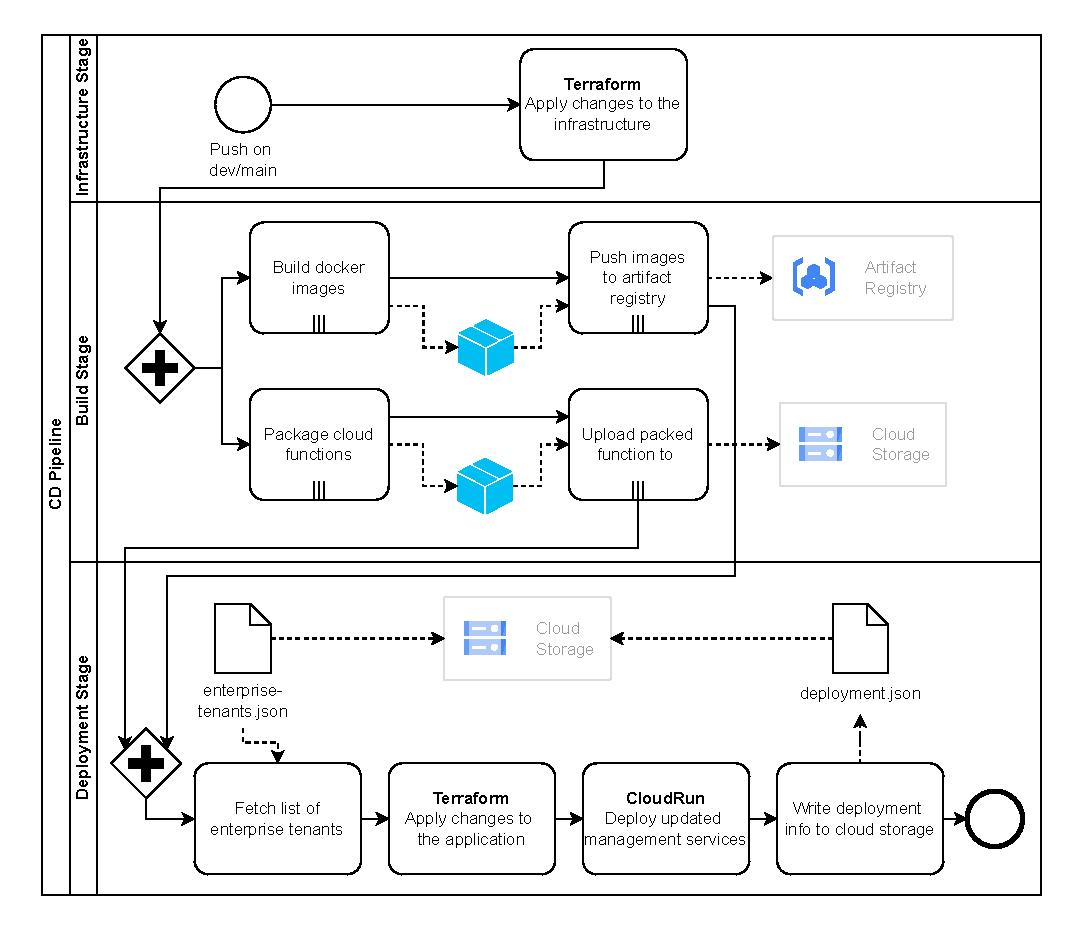
\includegraphics[width=\textwidth]{resources/cd-pipeline.pdf}
  \caption{CD Pipeline}
  \label{fig:cd-pipeline}
\end{figure}



\subsection{New Tenants}
\subsection{Monitoring}
\subsection{Load Testing}
\goodbreak
\section{Commercial Model}
\subsection{Tenant Types}

\paragraph{Free Tenant}
Der Free Plan richtet sich an Benutzer, die grundlegende Funktionen zur Verwaltung von Standorten und Infrastruktur benötigen. Die wesentlichen Merkmale dieses Plans umfassen:
\begin{itemize}
    \item \textbf{Parkhausverwaltung:} Erstellung und Management mehrerer Parkhäuser, um Standorte effizient zu organisieren.
    \item \textbf{Defektmanagement:} Nachverfolgung und Bearbeitung von Defekten, um eine schnelle Problemlösung zu gewährleisten.
    \item \textbf{Integration von eMobility-Ladestationen:} Einbindung und Überwachung von Ladeinfrastruktur für Elektrofahrzeuge.
\end{itemize}
Der Free Plan bietet die essenziellen Tools, um Parkhäuser und Ladestationen effizient zu managen, ohne dabei monatliche Kosten zu verursachen.

\paragraph{Premium Tenant}
Der Premium Plan hat die selbe Grundfunktionalität wie der Free Plan und richtet sich an Organisationen mit gesteigerten Anforderungen an Benutzerfreundlichkeit, Analysen und Leistung. 
Die Merkmale umfassen:
\begin{itemize}
    \item \textbf{Benutzerverwaltung:} Unbegrenzte Hinzufügung von Benutzern und umfassende Zugriffskontrolle.
    \item \textbf{eMobility-Ladestationen:} Einfache Integration und Verwaltung von Ladeinfrastruktur.
    \item \textbf{Mehrsprachigkeit:} Unterstützung für mehrere Sprachen zur Förderung internationaler Zusammenarbeit.
    \item \textbf{Analytics-Page:} Bereitstellung von detaillierten Analysen und Einblicken zur Optimierung der operativen Prozesse.
    \item \textbf{Verbesserte Performance:} Schnellere Ladezeiten und höhere Zuverlässigkeit des Systems.
    \item \textbf{Premium-Support:} Priorisierte Kundenbetreuung für schnelle Problemlösung.
    \item \textbf{Erhöhte Sicherheit:} Erweiterte Sicherheitsfeatures zum Schutz sensibler Daten.
\end{itemize}
\textbf{Kosten:}
\begin{itemize}
    \item \textbf{79,00 €/Monat} Grundgebühr.
    \item \textbf{1 €/Benutzer.}
    \item \textbf{5 €/10.000 Backend-Requests.}
\end{itemize}

\paragraph{Enterprise Tenant}
Der Enterprise Plan bietet die gleiche Funktionalität wie der Premium Plan, ist jedoch für große Organisationen ausgelegt, die maximale Leistung, Sicherheit und Unterstützung benötigen. 
Die enthaltenen Features bieten höchste Flexibilität und Effizienz:
\begin{itemize}
    \item \textbf{Anpassbarkeit:} Der Kunde erhält eigene Domain.
    \item \textbf{Beste Performance:} Höchste Geschwindigkeit und Systemzuverlässigkeit.
    \item \textbf{Top-Support:} Höchstpriorisierte Unterstützung für alle Anliegen.
    \item \textbf{Höchste Sicherheitsstandards:} Umfassender Schutz sensibler Daten.
\end{itemize}
\textbf{Kosten:}
\begin{itemize}
    \item \textbf{129,90 €/Monat} Grundgebühr.
    \item \textbf{5 €/10.000 Backend-Requests.}
\end{itemize}

\subsection{Pricing Model}
Die Preisstruktur der Plattform bietet flexible Modelle, die auf die unterschiedlichen Anforderungen der Benutzer zugeschnitten sind. 
Sie ermöglicht eine einfache Skalierbarkeit basierend auf der Anzahl der Benutzer und der Backend-Anfragen.

\begin{table}[h!]
\centering
\caption{Preisübersicht der Tenant Types}
\begin{tabular}{|l|c|c|c|}
\hline
\textbf{Plan}         & \textbf{Grundgebühr (€/Monat)} & \textbf{Preis pro Benutzer (€/Monat)} & \textbf{Preis pro 10.000 Backend-Requests (€/Monat)} \\ \hline
Free                  & 0,00                          & -                                    & -                                                   \\ \hline
Premium               & 79,00                         & 1,00                                 & 5,00                                                \\ \hline
Enterprise            & 129,90                        & -                                    & 5,00                                                \\ \hline
\end{tabular}
\label{tab:pricing}
\end{table}

Die Tabelle \ref{tab:pricing} fasst die Preise der verschiedenen Tenant Types zusammen und verdeutlicht die unterschiedlichen Kostenmodelle:

- Der \textit{Free Plan} ist kostenlos (0,00 €/Monat) und beinhaltet keine zusätzlichen Gebühren für Benutzer oder Backend-Anfragen. 
Er eignet sich ideal für kleine Teams oder Einzelpersonen, die grundlegende Funktionen benötigen, ohne Kosten zu verursachen.
  
- Der \textit{Premium Plan} bietet erweiterte Funktionen zu einer Grundgebühr von 79,00 €/Monat. 
Zusätzlich fällt ein flexibler Betrag von 1,00 € pro Benutzer und 5,00 € pro 10.000 Backend-Anfragen an, wodurch dieser Plan für mittelgroße Teams und Organisationen geeignet ist.

- Der \textit{Enterprise Plan} richtet sich an große Organisationen mit hohen Anforderungen. 
Die Grundgebühr beträgt 129,90 €/Monat, wobei die Kosten für Backend-Anfragen identisch zum Premium Plan sind (5,00 € pro 10.000 Backend-Anfragen). 
Eine Kostenstruktur pro Benutzer entfällt in diesem Plan, was ihn für Unternehmen mit einer großen Benutzerbasis besonders attraktiv macht.

Diese Preisgestaltung bietet die notwendige Flexibilität und Skalierbarkeit, um sowohl kleine als auch große Benutzergruppen effizient zu bedienen.

\subsection{Cost Model}
Das interne Kostenmodell basiert auf einer effizienten Ressourcennutzung und differenziert zwischen den Anforderungen der verschiedenen Tenant Types. Die Aufteilung der Ressourcen erfolgt wie folgt:

\begin{itemize}
    \item \textbf{Free Plan:} Alle Mandanten teilen sich einen Kubernetes-Namespace, eine gemeinsame Firestore-Datenbank und einen gemeinsamen Cloud Storage.
    \item \textbf{Premium Plan:} Mandanten teilen sich ebenfalls einen Kubernetes-Namespace, jedoch mit höheren Ressourcenallokationen, sowie eine gemeinsame Firestore-Datenbank und einen gemeinsamen Cloud Storage.
    \item \textbf{Enterprise Plan:} Jeder Mandant erhält einen eigenen Kubernetes-Namespace, eine eigene Firestore-Datenbank und einen eigenen Cloud Storage, um maximale Isolation und Leistung zu gewährleisten.
    \item \textbf{Geteilte Services:} Drei zentrale Services, die auf Google Cloud Run ausgeführt werden, werden von allen Mandanten gemeinsam genutzt, unabhängig vom Plan.
\end{itemize}

\begin{table}[h!]
\centering
\caption{Ressourcennutzung und Kostenschätzung pro Monat}
\begin{tabular}{|l|c|c|c|}
\hline
\textbf{Ressource}               & \textbf{Free Plan} & \textbf{Premium Plan} & \textbf{Enterprise (pro Mandant)} \\ \hline
Kubernetes Namespace             & 50 €/Monat         & 150 €/Monat           & 40 €/Monat                        \\ \hline
Firestore-Datenbank              & 30 €/Monat         & 100 €/Monat           & 10 €/Monat                        \\ \hline
Cloud Storage                    & 20 €/Monat         & 50 €/Monat            & 6 €/Monat                         \\ \hline
Cloud Run (geteilt)              & 100 €/Monat        & 200 €/Monat           & 40 €/Monat (anteilig)              \\ \hline
\textbf{Gesamtkosten (Schätzung)} & 200 €/Monat        & 500 €/Monat           & 96 €/Monat                        \\ \hline
\end{tabular}
\label{tab:costmodel}
\end{table}

In Tabelle \ref{tab:costmodel} werden die geschätzten Kosten für die verschiedenen Pläne dargestellt. Dabei wurden die ursprünglichen Kosten für den Enterprise Plan durch fünf geteilt, um die Verteilung der Ausgaben für einzelne Mandanten zu berücksichtigen. Die wichtigsten Punkte sind:

\begin{itemize}
    \item \textbf{Free Plan:} Die Gesamtkosten belaufen sich auf geschätzte 200 €/Monat durch die gemeinsame Nutzung von Ressourcen.
    \item \textbf{Premium Plan:} Durch höhere Anforderungen betragen die Kosten für alle Premium-Mandanten zusammen etwa 500 €/Monat.
    \item \textbf{Enterprise Plan:} Jeder Enterprise-Mandant verursacht individuelle Kosten von rund 96 €/Monat. Dies ist bedingt durch die exklusive Zuweisung von Ressourcen wie Kubernetes-Namespace, Firestore-Datenbank und Cloud Storage.
\end{itemize}

Dieses Kostenmodell bietet eine klare Grundlage für die wirtschaftliche Planung und Skalierung der Plattform.

\goodbreak
\section{Appendix}

\subsection{Mircoservice Configuration}
{\rowcolors{2}{}{gray!20}
\begin{longtable}{l p{6cm}}
  \caption{Environment-Variablen für den Authentication Service}
  \label{tab:auth-service-env-vars} \\
  \textbf{Environment-Variable} & \textbf{Beschreibung} \\ [1ex]
  \texttt{IDENTITY\_PLATFORM\_API\_KEY} & API-Schlüssel für die Identity Platform \\ [0.5ex]
  \texttt{IDENTITY\_PLATFORM\_AUTH\_DOMAIN} & Authentifizierungs-Domain für die Identity Platform \\ [0.5ex]
  \texttt{IDENTITY\_PLATFORM\_PROJECT\_ID} & Projekt-ID der Identity Platform \\ [0.5ex]
  \texttt{FIRESTORE\_DB\_ID} & Identifier für die Firestore-Datenbank \\ [0.5ex]
  \texttt{PORT} & Port, auf dem der Service läuft \\ [0.5ex]
  \texttt{INFRASTRUCTURE\_SERVICE\_URL} & URL für den Infrastructure Service \\ [0.5ex]
  \texttt{INFRASTRUCTURE\_ADMINISTRATION\_SERVICE\_AUDIENCE} & Zielgruppe des Administration Service \\ 
\end{longtable}}


% Infrastructure Administration Service Table
{\rowcolors{2}{}{gray!20}
\begin{longtable}{l p{6cm}}
  \caption{Environment-Variablen für den Infrastructure Administration Service}
  \label{tab:infra-admin-service-env-vars} \\
  \textbf{Environment-Variable} & \textbf{Beschreibung} \\ [1ex]
  \texttt{AUTHENTICATION\_SERVICE\_URL} & URL des Authentication Service \\ [0.5ex]
  \texttt{ANALYTICS\_DB\_ID} & Identifier für die Analytics-Datenbank \\ [0.5ex]
  \texttt{INFRASTRUCTURE\_ADMINISTRATION\_SERVICE\_AUDIENCE} & Zielgruppe des Administration Service \\ [0.5ex]
  \texttt{PORT} & Port, auf dem der Service läuft \\ [0.5ex]
  \texttt{GITHUB\_ACTION\_TOKEN} & Token für GitHub-Aktionen \\ [0.5ex]
  \texttt{GITHUB\_TENANT\_WORKFLOW\_ID} & ID des GitHub-Tenant-Workflows \\ [0.5ex]
  \texttt{GITHUB\_TENANT\_WORKFLOW\_BRANCH} & Branch für den GitHub-Tenant-Workflow \\ 
\end{longtable}}

% Parking Management Service Table
{\rowcolors{2}{}{gray!20}
\begin{longtable}{l p{6cm}}
  \caption{Environment-Variablen für den Parking Management Service}
  \label{tab:parking-mgmt-service-env-vars} \\
  \textbf{Environment-Variable} & \textbf{Beschreibung} \\ [1ex]
  \texttt{FIRESTORE\_DB\_ID} & Identifier für die Firestore-Datenbank \\ [0.5ex]
  \texttt{AUTHENTICATION\_SERVICE\_URL} & URL des Authentication Service \\ [0.5ex]
  \texttt{INFRASTRUCTURE\_MANAGEMENT\_SERVICE\_URL} & URL des Infrastructure Management Service \\ [0.5ex]
  \texttt{INFRASTRUCTURE\_ADMINISTRATION\_SERVICE\_AUDIENCE} & Zielgruppe des Administration Service \\ [0.5ex]
  \texttt{PORT} & Port, auf dem der Service läuft \\ 
\end{longtable}}

% Property Management Service Table
{\rowcolors{2}{}{gray!20}
\begin{longtable}{l p{6cm}}
  \caption{Environment-Variablen für den Property Management Service}
  \label{tab:property-mgmt-service-env-vars} \\
  \textbf{Environment-Variable} & \textbf{Beschreibung} \\ [1ex]
  \texttt{FIRESTORE\_DB\_ID} & Identifier für die Firestore-Datenbank \\ [0.5ex]
  \texttt{GCS\_BUCKET\_ID} & Identifier für den Google Cloud Storage Bucket \\ [0.5ex]
  \texttt{PARKING\_MANAGEMENT\_BACKEND\_URL} & URL des Parking Management Backends \\ [0.5ex]
  \texttt{AUTHENTICATION\_SERVICE\_URL} & URL des Authentication Service \\ [0.5ex]
  \texttt{INFRASTRUCTURE\_MANAGEMENT\_SERVICE\_URL} & URL des Infrastructure Management Service \\ [0.5ex]
  \texttt{INFRASTRUCTURE\_ADMINISTRATION\_SERVICE\_AUDIENCE} & Zielgruppe des Administration Service \\ [0.5ex]
  \texttt{PORT} & Port, auf dem der Service läuft \\ 
\end{longtable}}

% Park Frontend Table
{\rowcolors{2}{}{gray!20}
\begin{longtable}{l p{6cm}}
  \caption{Environment-Variablen für das Park Frontend}
  \label{tab:park-frontend-env-vars} \\
  \textbf{Environment-Variable} & \textbf{Beschreibung} \\ [1ex]
  \texttt{VITE\_TENANT\_ID} & ID des Tenants \\ [0.5ex]
  \texttt{VITE\_TENANT\_TYPE} & Typ des Tenants \\ [0.5ex]
  \texttt{VITE\_PROPERTY\_MANAGEMENT\_SERVICE\_URL} & URL des Property Management Services \\ [0.5ex]
  \texttt{VITE\_AUTHENTICATION\_SERVICE\_URL} & URL des Authentication Services \\ [0.5ex]
  \texttt{VITE\_PARKING\_MANAGEMENT\_SERVICE\_URL} & URL des Parking Management Services \\ [0.5ex]
  \texttt{VITE\_INFRASTRUCTURE\_MANAGEMENT\_SERVICE\_URL} & URL des Infrastructure Management Services \\ [0.5ex]
  \texttt{VITE\_IDENTITY\_PLATFORM\_API\_KEY} & API-Schlüssel für die Identity Platform \\ [0.5ex]
  \texttt{VITE\_IDENTITY\_PLATFORM\_AUTH\_DOMAIN} & Authentifizierungs-Domain für die Identity Platform \\ [0.5ex]
  \texttt{VITE\_IDENTITY\_PLATFORM\_PROJECT\_ID} & Projekt-ID der Identity Platform \\ 
\end{longtable}}

% Sign Up Frontend Table
{\rowcolors{2}{}{gray!20}
\begin{longtable}{l p{6cm}}
  \caption{Environment-Variablen für das Sign Up Frontend}
  \label{tab:signup-frontend-env-vars} \\
  \textbf{Environment-Variable} & \textbf{Beschreibung} \\ [1ex]
  \texttt{VITE\_AUTHENTICATION\_SERVICE\_URL} & URL des Authentication Services \\ 
\end{longtable}}
\goodbreak

\goodbreak

\end{sloppypar}
\end{document}
